% Options for packages loaded elsewhere
\PassOptionsToPackage{unicode}{hyperref}
\PassOptionsToPackage{hyphens}{url}
%
\documentclass[
]{article}
\usepackage{lmodern}
\usepackage{amssymb,amsmath}
\usepackage{ifxetex,ifluatex}
\ifnum 0\ifxetex 1\fi\ifluatex 1\fi=0 % if pdftex
  \usepackage[T1]{fontenc}
  \usepackage[utf8]{inputenc}
  \usepackage{textcomp} % provide euro and other symbols
\else % if luatex or xetex
  \usepackage{unicode-math}
  \defaultfontfeatures{Scale=MatchLowercase}
  \defaultfontfeatures[\rmfamily]{Ligatures=TeX,Scale=1}
\fi
% Use upquote if available, for straight quotes in verbatim environments
\IfFileExists{upquote.sty}{\usepackage{upquote}}{}
\IfFileExists{microtype.sty}{% use microtype if available
  \usepackage[]{microtype}
  \UseMicrotypeSet[protrusion]{basicmath} % disable protrusion for tt fonts
}{}
\makeatletter
\@ifundefined{KOMAClassName}{% if non-KOMA class
  \IfFileExists{parskip.sty}{%
    \usepackage{parskip}
  }{% else
    \setlength{\parindent}{0pt}
    \setlength{\parskip}{6pt plus 2pt minus 1pt}}
}{% if KOMA class
  \KOMAoptions{parskip=half}}
\makeatother
\usepackage{xcolor}
\IfFileExists{xurl.sty}{\usepackage{xurl}}{} % add URL line breaks if available
\IfFileExists{bookmark.sty}{\usepackage{bookmark}}{\usepackage{hyperref}}
\hypersetup{
  pdftitle={Team Project: Data Analysis Project Report: Consumer Attractions In Social Network Era},
  pdfauthor={Jianye Han (jianyeh2), Zach Litz (zlitz2), Megan Masanz (mjneuman)},
  hidelinks,
  pdfcreator={LaTeX via pandoc}}
\urlstyle{same} % disable monospaced font for URLs
\usepackage[margin=1in]{geometry}
\usepackage{color}
\usepackage{fancyvrb}
\newcommand{\VerbBar}{|}
\newcommand{\VERB}{\Verb[commandchars=\\\{\}]}
\DefineVerbatimEnvironment{Highlighting}{Verbatim}{commandchars=\\\{\}}
% Add ',fontsize=\small' for more characters per line
\usepackage{framed}
\definecolor{shadecolor}{RGB}{248,248,248}
\newenvironment{Shaded}{\begin{snugshade}}{\end{snugshade}}
\newcommand{\AlertTok}[1]{\textcolor[rgb]{0.94,0.16,0.16}{#1}}
\newcommand{\AnnotationTok}[1]{\textcolor[rgb]{0.56,0.35,0.01}{\textbf{\textit{#1}}}}
\newcommand{\AttributeTok}[1]{\textcolor[rgb]{0.77,0.63,0.00}{#1}}
\newcommand{\BaseNTok}[1]{\textcolor[rgb]{0.00,0.00,0.81}{#1}}
\newcommand{\BuiltInTok}[1]{#1}
\newcommand{\CharTok}[1]{\textcolor[rgb]{0.31,0.60,0.02}{#1}}
\newcommand{\CommentTok}[1]{\textcolor[rgb]{0.56,0.35,0.01}{\textit{#1}}}
\newcommand{\CommentVarTok}[1]{\textcolor[rgb]{0.56,0.35,0.01}{\textbf{\textit{#1}}}}
\newcommand{\ConstantTok}[1]{\textcolor[rgb]{0.00,0.00,0.00}{#1}}
\newcommand{\ControlFlowTok}[1]{\textcolor[rgb]{0.13,0.29,0.53}{\textbf{#1}}}
\newcommand{\DataTypeTok}[1]{\textcolor[rgb]{0.13,0.29,0.53}{#1}}
\newcommand{\DecValTok}[1]{\textcolor[rgb]{0.00,0.00,0.81}{#1}}
\newcommand{\DocumentationTok}[1]{\textcolor[rgb]{0.56,0.35,0.01}{\textbf{\textit{#1}}}}
\newcommand{\ErrorTok}[1]{\textcolor[rgb]{0.64,0.00,0.00}{\textbf{#1}}}
\newcommand{\ExtensionTok}[1]{#1}
\newcommand{\FloatTok}[1]{\textcolor[rgb]{0.00,0.00,0.81}{#1}}
\newcommand{\FunctionTok}[1]{\textcolor[rgb]{0.00,0.00,0.00}{#1}}
\newcommand{\ImportTok}[1]{#1}
\newcommand{\InformationTok}[1]{\textcolor[rgb]{0.56,0.35,0.01}{\textbf{\textit{#1}}}}
\newcommand{\KeywordTok}[1]{\textcolor[rgb]{0.13,0.29,0.53}{\textbf{#1}}}
\newcommand{\NormalTok}[1]{#1}
\newcommand{\OperatorTok}[1]{\textcolor[rgb]{0.81,0.36,0.00}{\textbf{#1}}}
\newcommand{\OtherTok}[1]{\textcolor[rgb]{0.56,0.35,0.01}{#1}}
\newcommand{\PreprocessorTok}[1]{\textcolor[rgb]{0.56,0.35,0.01}{\textit{#1}}}
\newcommand{\RegionMarkerTok}[1]{#1}
\newcommand{\SpecialCharTok}[1]{\textcolor[rgb]{0.00,0.00,0.00}{#1}}
\newcommand{\SpecialStringTok}[1]{\textcolor[rgb]{0.31,0.60,0.02}{#1}}
\newcommand{\StringTok}[1]{\textcolor[rgb]{0.31,0.60,0.02}{#1}}
\newcommand{\VariableTok}[1]{\textcolor[rgb]{0.00,0.00,0.00}{#1}}
\newcommand{\VerbatimStringTok}[1]{\textcolor[rgb]{0.31,0.60,0.02}{#1}}
\newcommand{\WarningTok}[1]{\textcolor[rgb]{0.56,0.35,0.01}{\textbf{\textit{#1}}}}
\usepackage{longtable,booktabs}
% Correct order of tables after \paragraph or \subparagraph
\usepackage{etoolbox}
\makeatletter
\patchcmd\longtable{\par}{\if@noskipsec\mbox{}\fi\par}{}{}
\makeatother
% Allow footnotes in longtable head/foot
\IfFileExists{footnotehyper.sty}{\usepackage{footnotehyper}}{\usepackage{footnote}}
\makesavenoteenv{longtable}
\usepackage{graphicx,grffile}
\makeatletter
\def\maxwidth{\ifdim\Gin@nat@width>\linewidth\linewidth\else\Gin@nat@width\fi}
\def\maxheight{\ifdim\Gin@nat@height>\textheight\textheight\else\Gin@nat@height\fi}
\makeatother
% Scale images if necessary, so that they will not overflow the page
% margins by default, and it is still possible to overwrite the defaults
% using explicit options in \includegraphics[width, height, ...]{}
\setkeys{Gin}{width=\maxwidth,height=\maxheight,keepaspectratio}
% Set default figure placement to htbp
\makeatletter
\def\fps@figure{htbp}
\makeatother
\setlength{\emergencystretch}{3em} % prevent overfull lines
\providecommand{\tightlist}{%
  \setlength{\itemsep}{0pt}\setlength{\parskip}{0pt}}
\setcounter{secnumdepth}{-\maxdimen} % remove section numbering

\title{Team Project: Data Analysis Project Report: Consumer Attractions In
Social Network Era}
\author{Jianye Han (jianyeh2), Zach Litz (zlitz2), Megan Masanz (mjneuman)}
\date{July 29, 2017}

\begin{document}
\maketitle

\hypertarget{i.-introduction}{%
\section{\texorpdfstring{\textbf{I}.
Introduction}{I. Introduction}}\label{i.-introduction}}

In this project, we will be examining a dataset {[}1{]} that contains
social media information for a particular cosmetics brand. The data
contains information about posts that were published on the brand's
Facebook page during the year of 2014. There are approximately 500
records in this dataset (prior to any cleaning).

The information includes what would be expected from social media page
metrics such as \texttt{Page\ total\ like},
\texttt{Lifetime\ Post\ Consumption}, \texttt{Total\ Interactions},
\texttt{Post\ Month}, and \texttt{Type} (see {[}Table A.1{]} for a
complete list of variables).

We are particularly interested in the variable
\texttt{Lifetime\ Post\ Consumers}. This variable gives the total number
of clicks anywhere in a post over the post's lifetime. Our goal is to
create a multiple regression model that explains the
\texttt{Lifetime\ Post\ Consumers} variable based on the other
variables.

It is widely understood that Facebook marketing is an important tool
used by modern data businesses in order to create social awareness and
increase revenue. For this project, we are operating under the
assumption that \texttt{Lifetime\ Post\ Consumers} is a good metric for
evaluating how effective a Facebook post is in achieving advertising
goals. In other words, a large value for
\texttt{Lifetime\ Post\ Consumers} corresponds to a high social
awareness which can lead to increased revenue. Thus, it seems to be
beneficial to understand how \texttt{Lifetime\ Post\ Consumers} is
explained by the other variables in the dataset in an effort to increase
\texttt{Lifetime\ Post\ Consumers}.

Because our goal is to explain \texttt{Lifetime\ Post\ Consumers}, we
will try to find the smallest model that gives good results. We are
interested in a smaller and simpler model in order to ensure the model
is understandable. To do this, we will use various techniques for model
selection and quality criteria. These techniques will be described in
the methods section.

\hypertarget{ii.-methods}{%
\section{\texorpdfstring{\textbf{II}.
Methods}{II. Methods}}\label{ii.-methods}}

The first step in our analysis is to prepare the data. The data is
prepared as follows:

\begin{enumerate}
\def\labelenumi{\arabic{enumi}.}
\tightlist
\item
  Remove all incomplete records. For our purposes, an incomplete record
  is any record which has empty or NA values. This steps results in a
  total of 5 records being removed.\\
\item
  Convert numeric categorical variables to proper factors. We convert

  \begin{itemize}
  \tightlist
  \item
    \texttt{Type}~\\
  \item
    \texttt{Category}~\\
  \item
    \texttt{Post\ Month}~\\
  \item
    \texttt{Post\ Hours}~\\
  \item
    \texttt{Post\ Weekday}~\\
  \item
    \texttt{Paid}~\\
  \end{itemize}
\item
  Remove the \texttt{Total\ Interactions} variable because it is
  perfectly correlated with the response.
\end{enumerate}

\hypertarget{variable-exploration}{%
\subsubsection{Variable Exploration}\label{variable-exploration}}

\hypertarget{the-additive-model}{%
\paragraph{The Additive Model}\label{the-additive-model}}

Our first step into exploring and analyzing this data is to create a
full additive model. This additive model will include all predictors in
the dataset. There are no transformations or interactions. (See {[}Table
A.1{]} for a complete description of variables). The response variable
is \texttt{Lifetime\ Post\ Consumers}.

\begin{Shaded}
\begin{Highlighting}[]
\NormalTok{full_additive_model <-}\StringTok{ }\KeywordTok{lm}\NormalTok{(Lifetime.Post.Consumers }\OperatorTok{~}\StringTok{ }\NormalTok{., }\DataTypeTok{data =}\NormalTok{ complete_data)}
\end{Highlighting}
\end{Shaded}

We begin our analysis by trying to develop an understanding of how the
predictor variables relate to each other. Here we will look at \(R^2_j\)
and the variance inflation factor (VIF). This information will help us
understand the effect of collinearity on the variance of the regression
estimates, as well as the proportion of observed variation each
predictor as explained by the other predictors. {[}Table 2.1{]} shows
the \(R^2_j\) and VIF values for each applicable predictor used in the
fully additive model (note that categorical predictors have \texttt{NA}
values).

\#\#\#\#Table 2.1

\begin{longtable}[]{@{}lrr@{}}
\caption{Table 2.1 - Rj\^{}2 and VIF values for full additive
model}\tabularnewline
\toprule
predictor & rj\_squared & vif\tabularnewline
\midrule
\endfirsthead
\toprule
predictor & rj\_squared & vif\tabularnewline
\midrule
\endhead
Page.total.likes & 0.99 & 154.6\tabularnewline
Type & NA & NA\tabularnewline
Category & NA & NA\tabularnewline
Post.Month & NA & NA\tabularnewline
Post.Weekday & NA & NA\tabularnewline
Post.Hour & NA & NA\tabularnewline
Paid & NA & NA\tabularnewline
Lifetime.Post.Total.Reach & 0.96 & 24.2\tabularnewline
Lifetime.Post.Total.Impressions & 0.97 & 35.4\tabularnewline
Lifetime.Engaged.Users & 0.89 & 9.3\tabularnewline
Lifetime.Post.Consumptions & 0.61 & 2.6\tabularnewline
Lifetime.Post.Impressions.by.people.who.have.liked.your.Page & 0.96 &
24.8\tabularnewline
Lifetime.Post.reach.by.people.who.like.your.Page & 0.91 &
11.6\tabularnewline
Lifetime.People.who.have.liked.your.Page.and.engaged.with.your.post &
0.89 & 9.5\tabularnewline
comment & 0.81 & 5.3\tabularnewline
like & 0.91 & 11.1\tabularnewline
share & 0.90 & 9.6\tabularnewline
\bottomrule
\end{longtable}

The high \(R^2_j\) values in {[}Table 2.1{]} show that each given
predictor can be explained by other predictors. This suggest that we can
remove some of the predictors from this model. The high VIF values
indicate that our estimates of the \(\beta\) parameters are going to be
highly variable. This high variability is undesirable given our goal of
using the model for explanation. Having established that this is a poor
model for explanation, we will begin to simplify the model.

\hypertarget{additive-model-selection}{%
\paragraph{Additive Model Selection}\label{additive-model-selection}}

We will start the selection process by using the R \texttt{step()}
function to perform forward and backward searches. In addition to doing
AIC and BIC searches, we will also do a forward search using 0 penalty
which means only RSS matters (lower RSS wins). Instead of taking the
model returned by the \texttt{step()} function, we will keep a list of
the models selected at each step. Then we will perform ANOVA F-tests for
each group of models to find the smallest model that is significant.
This will give us the five models described in table 2.2. We will then
find the best model from this group which will be used for the next
step.

\#\#\#\#Table 2.2

\begin{longtable}[]{@{}ll@{}}
\caption{Table 2.2 - Model Selection Description}\tabularnewline
\toprule
Model & Description\tabularnewline
\midrule
\endfirsthead
\toprule
Model & Description\tabularnewline
\midrule
\endhead
rss\_fwd\_model & Smallest significant model found using forward search
with no penalty\tabularnewline
aic\_fwd\_model & Smallest significant model found using forward search
with penalty 2P\tabularnewline
bic\_fwd\_model & Smallest significant model found using forward search
with penalty log(n)\tabularnewline
aic\_bwd\_model & Smallest significant model found using backward search
with penalty 2p\tabularnewline
bic\_bwd\_model & Smallest significant model found using backward search
with penalty log(n)\tabularnewline
\bottomrule
\end{longtable}

Running through this process gives us five models.

The \texttt{rss\_fwd\_model} (which uses the forward selection process
with no penalty, meaning only RSS matters) has the predictors:

\begin{verbatim}
Lifetime.Engaged.Users + like + share + Lifetime.People.who.have.liked.your.Page.and.engaged.with.your.post + 
    Post.Month + Lifetime.Post.Consumptions + comment + Lifetime.Post.Total.Reach
\end{verbatim}

The \texttt{aic\_fwd\_model} has the predictors:

\begin{verbatim}
Lifetime.Engaged.Users + like + share + Lifetime.People.who.have.liked.your.Page.and.engaged.with.your.post + 
    Lifetime.Post.Consumptions + Post.Month + comment + Lifetime.Post.Total.Reach + 
    Type + Lifetime.Post.Total.Impressions + Lifetime.Post.Impressions.by.people.who.have.liked.your.Page
\end{verbatim}

The \texttt{bic\_fwd\_model} has the predictors:

\begin{verbatim}
Lifetime.Engaged.Users + like + share + Lifetime.People.who.have.liked.your.Page.and.engaged.with.your.post + 
    Lifetime.Post.Consumptions + comment + Page.total.likes + 
    Lifetime.Post.Total.Reach
\end{verbatim}

The \texttt{aic\_bwd\_model} has the predictors:

\begin{verbatim}
Type + Post.Month + Lifetime.Post.Total.Reach + Lifetime.Post.Total.Impressions + 
    Lifetime.Engaged.Users + Lifetime.Post.Consumptions + Lifetime.Post.Impressions.by.people.who.have.liked.your.Page + 
    Lifetime.People.who.have.liked.your.Page.and.engaged.with.your.post + 
    comment + like + share
\end{verbatim}

The \texttt{bic\_bwd\_model} has the predictors:

\begin{verbatim}
Page.total.likes + Lifetime.Post.Total.Reach + Lifetime.Post.Total.Impressions + 
    Lifetime.Engaged.Users + Lifetime.Post.Consumptions + Lifetime.People.who.have.liked.your.Page.and.engaged.with.your.post + 
    comment + like + share
\end{verbatim}

Once again, we will look at the \(R^2_j\) and VIF values for the models.
{[}Table 2.3{]}, {[}Table 2.4{]}, {[}Table 2.5{]}, {[}Table 2.6{]}, and
{[}Table 2.7{]} show these values for the \texttt{rss\_fwd\_model},
\texttt{aic\_fwd\_model}, \texttt{bic\_fwd\_model},
\texttt{aic\_bwd\_model}, and \texttt{bic\_bwd\_model} respectively.

Note that the categorical variables will be displayed in the table as
\texttt{NA}, this is due to the fact that these predictors will add many
variables into the model. For a categorical variable with k categories,
it will introduce k-1 predictor variables, so for simplicity of
analysis, these will be looked at seperately during our analysis in
section \protect\hyperlink{categorical-predictors}{Categorical
Predictors}.

\#\#\#\#Table 2.3

\begin{longtable}[]{@{}lrr@{}}
\caption{Table 2.3 - Rj\^{}2 and VIF values for
rss\_fwd\_model}\tabularnewline
\toprule
predictor & rj\_squared & vif\tabularnewline
\midrule
\endfirsthead
\toprule
predictor & rj\_squared & vif\tabularnewline
\midrule
\endhead
Lifetime.Engaged.Users & 0.84 & 6.1\tabularnewline
like & 0.86 & 7.2\tabularnewline
share & 0.87 & 7.9\tabularnewline
Lifetime.People.who.have.liked.your.Page.and.engaged.with.your.post &
0.74 & 3.8\tabularnewline
Post.Month & NA & NA\tabularnewline
Lifetime.Post.Consumptions & 0.53 & 2.1\tabularnewline
comment & 0.78 & 4.6\tabularnewline
Lifetime.Post.Total.Reach & 0.45 & 1.8\tabularnewline
\bottomrule
\end{longtable}

\#\#\#\#Table 2.4

\begin{longtable}[]{@{}lrr@{}}
\caption{Table 2.4 - Rj\^{}2 and VIF values for
aic\_fwd\_model}\tabularnewline
\toprule
predictor & rj\_squared & vif\tabularnewline
\midrule
\endfirsthead
\toprule
predictor & rj\_squared & vif\tabularnewline
\midrule
\endhead
Lifetime.Engaged.Users & 0.85 & 6.5\tabularnewline
like & 0.90 & 9.6\tabularnewline
share & 0.89 & 8.8\tabularnewline
Lifetime.People.who.have.liked.your.Page.and.engaged.with.your.post &
0.83 & 6.0\tabularnewline
Lifetime.Post.Consumptions & 0.54 & 2.2\tabularnewline
Post.Month & NA & NA\tabularnewline
comment & 0.79 & 4.7\tabularnewline
Lifetime.Post.Total.Reach & 0.89 & 9.1\tabularnewline
Type & NA & NA\tabularnewline
Lifetime.Post.Total.Impressions & 0.95 & 19.5\tabularnewline
Lifetime.Post.Impressions.by.people.who.have.liked.your.Page & 0.91 &
11.2\tabularnewline
\bottomrule
\end{longtable}

\#\#\#\#Table 2.5

\begin{longtable}[]{@{}lrr@{}}
\caption{Table 2.5 - Rj\^{}2 and VIF values for
bic\_fwd\_model}\tabularnewline
\toprule
predictor & rj\_squared & vif\tabularnewline
\midrule
\endfirsthead
\toprule
predictor & rj\_squared & vif\tabularnewline
\midrule
\endhead
Lifetime.Engaged.Users & 0.83 & 6.0\tabularnewline
like & 0.86 & 7.0\tabularnewline
share & 0.87 & 7.5\tabularnewline
Lifetime.People.who.have.liked.your.Page.and.engaged.with.your.post &
0.73 & 3.7\tabularnewline
Lifetime.Post.Consumptions & 0.51 & 2.0\tabularnewline
comment & 0.78 & 4.5\tabularnewline
Page.total.likes & 0.10 & 1.1\tabularnewline
Lifetime.Post.Total.Reach & 0.43 & 1.8\tabularnewline
\bottomrule
\end{longtable}

\#\#\#\#Table 2.6

\begin{longtable}[]{@{}lrr@{}}
\caption{Table 2.6 - Rj\^{}2 and VIF values for
aic\_bwd\_model}\tabularnewline
\toprule
predictor & rj\_squared & vif\tabularnewline
\midrule
\endfirsthead
\toprule
predictor & rj\_squared & vif\tabularnewline
\midrule
\endhead
Type & NA & NA\tabularnewline
Post.Month & NA & NA\tabularnewline
Lifetime.Post.Total.Reach & 0.89 & 9.1\tabularnewline
Lifetime.Post.Total.Impressions & 0.95 & 19.5\tabularnewline
Lifetime.Engaged.Users & 0.85 & 6.5\tabularnewline
Lifetime.Post.Consumptions & 0.54 & 2.2\tabularnewline
Lifetime.Post.Impressions.by.people.who.have.liked.your.Page & 0.91 &
11.2\tabularnewline
Lifetime.People.who.have.liked.your.Page.and.engaged.with.your.post &
0.83 & 6.0\tabularnewline
comment & 0.79 & 4.7\tabularnewline
like & 0.90 & 9.6\tabularnewline
share & 0.89 & 8.8\tabularnewline
\bottomrule
\end{longtable}

\#\#\#\#Table 2.7

\begin{longtable}[]{@{}lrr@{}}
\caption{Table 2.7 - Rj\^{}2 and VIF values for
bic\_bwd\_model}\tabularnewline
\toprule
predictor & rj\_squared & vif\tabularnewline
\midrule
\endfirsthead
\toprule
predictor & rj\_squared & vif\tabularnewline
\midrule
\endhead
Page.total.likes & 0.12 & 1.1\tabularnewline
Lifetime.Post.Total.Reach & 0.67 & 3.0\tabularnewline
Lifetime.Post.Total.Impressions & 0.52 & 2.1\tabularnewline
Lifetime.Engaged.Users & 0.84 & 6.2\tabularnewline
Lifetime.Post.Consumptions & 0.51 & 2.0\tabularnewline
Lifetime.People.who.have.liked.your.Page.and.engaged.with.your.post &
0.74 & 3.9\tabularnewline
comment & 0.78 & 4.6\tabularnewline
like & 0.86 & 7.0\tabularnewline
share & 0.87 & 7.5\tabularnewline
\bottomrule
\end{longtable}

We can see in tables 2.4 to 2.7 that the variance inflation factors are
greatly improved. If we consider a VIF larger than 5 to indicate
mulitcollinearity issues, then we can count the number of large VIFs for
each models as:

\begin{itemize}
\tightlist
\item
  \texttt{rss\_fwd\_model}: 4 VIFs greater than 5
\item
  \texttt{aic\_fwd\_model}: 9 VIFs greater than 5
\item
  \texttt{bic\_fwd\_model}: 3 VIFs greater than 5
\item
  \texttt{aic\_bwd\_model}: 9 VIFs greater than 5
\item
  \texttt{bic\_bwd\_model}: 3 VIFs greater than 5
\end{itemize}

It is easy to see that all of the models have much less collinearity
issues than the original full additive model (based on the much smaller
VIF values).

Given both the \texttt{rss\_fwd\_model} and the \texttt{aic\_fwd\_model}
model included \texttt{Post.Month} as a categorical variable that was
included in the model, we will explore introducing this categorical
variable into the model and the possibility of interaction with the
other variables.

Table 2.8 shows the variables included in each of the five models.

\#\#\#\#Table 2.8

\begin{longtable}[]{@{}llllll@{}}
\caption{Table 2.8 - MLR Additive Model Variable
Analysis}\tabularnewline
\toprule
Variable & RSS Forward & AIC Forward & BIC Forward & AIC Backward & BIC
Backward\tabularnewline
\midrule
\endfirsthead
\toprule
Variable & RSS Forward & AIC Forward & BIC Forward & AIC Backward & BIC
Backward\tabularnewline
\midrule
\endhead
Page.total.likes & FALSE & FALSE & TRUE & FALSE & TRUE\tabularnewline
Type & FALSE & TRUE & FALSE & TRUE & FALSE\tabularnewline
Category & FALSE & FALSE & FALSE & FALSE & FALSE\tabularnewline
Post.Month & TRUE & TRUE & FALSE & TRUE & FALSE\tabularnewline
Post.Weekday & FALSE & FALSE & FALSE & FALSE & FALSE\tabularnewline
Post.Hour & FALSE & FALSE & FALSE & FALSE & FALSE\tabularnewline
Paid & FALSE & FALSE & FALSE & FALSE & FALSE\tabularnewline
Lifetime.Post.Total.Reach & TRUE & TRUE & TRUE & TRUE &
TRUE\tabularnewline
Lifetime.Post.Total.Impressions & FALSE & TRUE & FALSE & TRUE &
TRUE\tabularnewline
Lifetime.Engaged.Users & TRUE & TRUE & TRUE & TRUE & TRUE\tabularnewline
Lifetime.Post.Consumptions & TRUE & TRUE & TRUE & TRUE &
TRUE\tabularnewline
Lifetime.Post.Impressions.by.people.who.have.liked.your.Page & FALSE &
TRUE & FALSE & TRUE & FALSE\tabularnewline
Lifetime.Post.reach.by.people.who.like.your.Page & FALSE & FALSE & FALSE
& FALSE & FALSE\tabularnewline
Lifetime.People.who.have.liked.your.Page.and.engaged.with.your.post &
TRUE & TRUE & TRUE & TRUE & TRUE\tabularnewline
comment & TRUE & TRUE & TRUE & TRUE & TRUE\tabularnewline
like & TRUE & TRUE & TRUE & TRUE & TRUE\tabularnewline
share & TRUE & TRUE & TRUE & TRUE & TRUE\tabularnewline
\bottomrule
\end{longtable}

{[}Table 2.8{]} gives us more of an idea on which variables should be
used in our analysis. We will look at these variables more closely by
creating a pairs plot that includes only the variables that are common
to all models.

\begin{figure}

{\centering 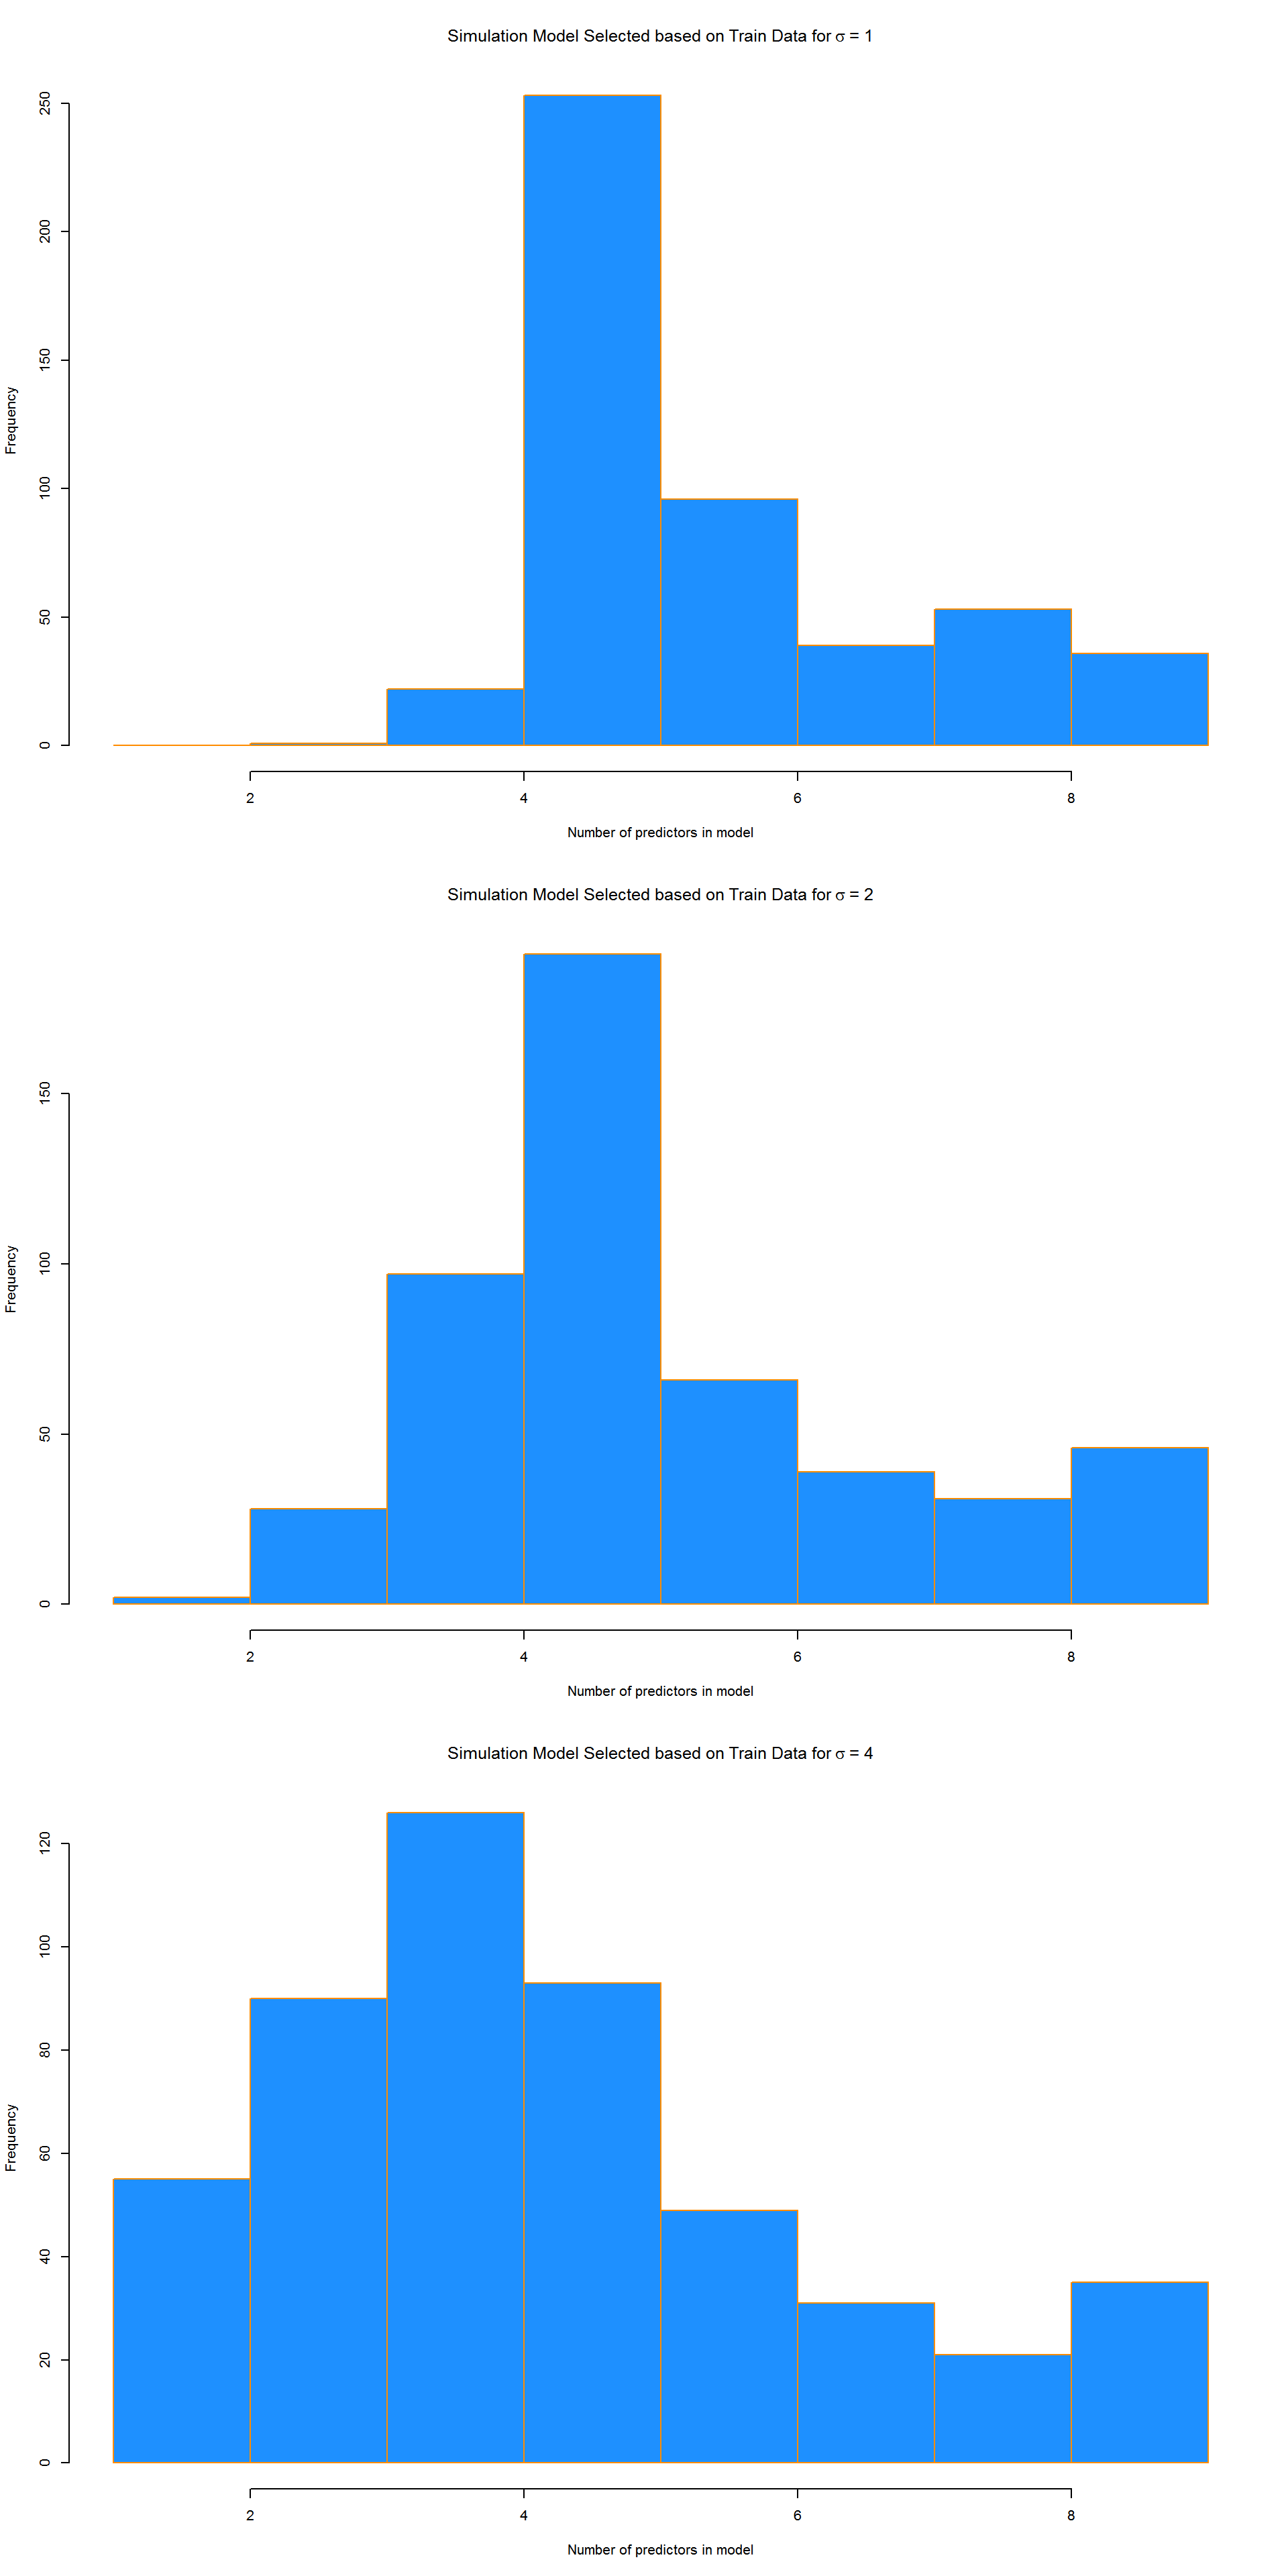
\includegraphics{report_3b_files/figure-latex/unnamed-chunk-20-1} 

}

\caption{Figure 2.1 - Pairs Plot of Important Variables}\label{fig:unnamed-chunk-20}
\end{figure}

While the pairs plot provide an idea regarding the variables of
interest.{[}Table 2.8{]} highlights we have 5 key variables of interest
that are not categorical predictors. These include

\begin{itemize}
\tightlist
\item
  share
\item
  like
\item
  comment
\item
  Lifetime.People.who.have.liked.your.Page.and.engaged.with.your.post
\item
  Lifetime.Engaged.Users
\end{itemize}

There are 2 variables we should explore futher namely: -
Lifetime.Post.Impressions.by.people.who.have.liked.your.Page -
Lifetime.Post.reach.by.people.who.like.your.Page

The 2 variables listed above were found in the \texttt{AIC\ Forward},
\texttt{BIC\ Forward}, \texttt{AIC\ Backward} and \texttt{BIC\ Backward}
models, but not in the \texttt{RSS\ Forward} model. To better understand
these variables we can look at a variables added plot to help understand
if these predictors should be considered with further investigation.

\begin{Shaded}
\begin{Highlighting}[]
\NormalTok{PostImpressionsModel =}\StringTok{ }\KeywordTok{lm}\NormalTok{(Lifetime.Post.Impressions.by.people.who.have.liked.your.Page }\OperatorTok{~}\StringTok{ }
\StringTok{                        }\NormalTok{Lifetime.Engaged.Users }\OperatorTok{+}\StringTok{ }\NormalTok{like }\OperatorTok{+}\StringTok{ }
\StringTok{                        }\NormalTok{share }\OperatorTok{+}\StringTok{ }\NormalTok{Lifetime.People.who.have.liked.your.Page.and.engaged.with.your.post }\OperatorTok{+}\StringTok{ }
\StringTok{                        }\NormalTok{comment, }\DataTypeTok{data  =}\NormalTok{ complete_data)}

\NormalTok{ModelWOutImpressions =}\StringTok{ }\KeywordTok{lm}\NormalTok{(Lifetime.Post.Consumers  }\OperatorTok{~}\StringTok{ }\NormalTok{Lifetime.Engaged.Users }\OperatorTok{+}\StringTok{ }\NormalTok{like }\OperatorTok{+}\StringTok{ }
\StringTok{                            }\NormalTok{share }\OperatorTok{+}\StringTok{ }\NormalTok{Lifetime.People.who.have.liked.your.Page.and.engaged.with.your.post }
                          \OperatorTok{+}\StringTok{ }\NormalTok{comment, }\DataTypeTok{data  =}\NormalTok{ complete_data)}
\end{Highlighting}
\end{Shaded}

\texttt{\{r.echo=FALSE,\ fig.width=10,\ fig.cap="\ Figure\ 2.1\ -\ Fitted\ vs\ Residual\ Plots\ for\ adding\ Lifetime.Post.Impressions.by.people.who.have.liked.your.Page",\ fig.align="center"\}\ plot(resid(ModelWOutImpressions)\ \textasciitilde{}\ resid(PostImpressionsModel),\ col\ =\ "dodgerblue",\ pch\ =\ 20,\ \ \ \ \ \ xlab\ =\ "Residuals,\ Added\ Predictor",\ ylab\ =\ "Residuals,\ Original\ Model")\ abline(h\ =\ 0,\ lty\ =\ 2)\ abline(v\ =\ 0,\ lty\ =\ 2)\ abline(lm(resid(ModelWOutImpressions)\ \textasciitilde{}\ resid(PostImpressionsModel)),\ \ \ \ \ \ \ \ col\ =\ "darkorange",\ lwd\ =\ 2)}

The partial correlation coefficient of
\texttt{Lifetime.Post.Impressions.by.people.who.have.liked.your.Page}
and \texttt{Lifetime.Post.Consumers} with the effects of the other
variables in the model removed with a value of 0.05 serves as additional
justication that this predictors should not end up in our final selected
model.

\begin{Shaded}
\begin{Highlighting}[]
\KeywordTok{cor}\NormalTok{(}\KeywordTok{resid}\NormalTok{(PostImpressionsModel), }\KeywordTok{resid}\NormalTok{(ModelWOutImpressions))}
\end{Highlighting}
\end{Shaded}

\begin{verbatim}
## [1] 0.046
\end{verbatim}

Futher investigation on
\texttt{Lifetime.Post.reach.by.people.who.like.your.Page}
```\{r.echo=FALSE, fig.width=10, fig.cap=" Figure 2.2 - Fitted vs
Residual Plots for adding
Lifetime.Post.reach.by.people.who.like.your.Page``,
fig.align=''center"\}

PostReachbyPeople = lm(Lifetime.Post.reach.by.people.who.like.your.Page
\textasciitilde{} Lifetime.Engaged.Users + like + share +
Lifetime.People.who.have.liked.your.Page.and.engaged.with.your.post +
comment, data = complete\_data)

ModelWOutPostReachbyPeople = lm(Lifetime.Post.Consumers
\textasciitilde{} Lifetime.Engaged.Users + like + share +
Lifetime.People.who.have.liked.your.Page.and.engaged.with.your.post +
comment, data = complete\_data)

plot(resid(ModelWOutPostReachbyPeople) \textasciitilde{}
resid(PostReachbyPeople), col = ``dodgerblue'', pch = 20, xlab =
``Residuals, Added Predictor'', ylab = ``Residuals, Original Model'')
abline(h = 0, lty = 2) abline(v = 0, lty = 2)
abline(lm(resid(ModelWOutPostReachbyPeople) \textasciitilde{}
resid(PostReachbyPeople)), col = ``darkorange'', lwd = 2)

\begin{verbatim}



```r
#cor(resid(PostReachbyPeople), resid(ModelWOutPostReachbyPeople))
\end{verbatim}

This information provide clarity that we should exclude these two
predictor variables from further analysis.

\hypertarget{categorical-predictors}{%
\paragraph{Categorical Predictors}\label{categorical-predictors}}

Both the \texttt{rss\_fwd\_model} and the \texttt{aic\_fwd\_model}
included \texttt{Post.Month} as a possible predictor. Below we consider
the \texttt{rss\_fwd\_model} as the \texttt{full\_model} and an MLR
model without Post.Month as the null model and confirm that the
preferred model does include the predictor \texttt{Post.Month}, however,
looking at the p-values for each of the individual dummy variables in
the model for Post.Month - we see that with the other predictors in the
model, these are not actually significant.

\begin{Shaded}
\begin{Highlighting}[]
\NormalTok{null_model =}\StringTok{ }\KeywordTok{lm}\NormalTok{(Lifetime.Post.Consumers }\OperatorTok{~}\StringTok{ }\NormalTok{Lifetime.Engaged.Users }\OperatorTok{+}\StringTok{ }\NormalTok{like }\OperatorTok{+}\StringTok{ }
\StringTok{                  }\NormalTok{share }\OperatorTok{+}\StringTok{ }\NormalTok{Lifetime.People.who.have.liked.your.Page.and.engaged.with.your.post }\OperatorTok{+}
\StringTok{                  }\NormalTok{comment, }\DataTypeTok{data =}\NormalTok{ complete_data)}

\NormalTok{full_model =}\StringTok{ }\KeywordTok{lm}\NormalTok{(Lifetime.Post.Consumers }\OperatorTok{~}\StringTok{ }\NormalTok{Lifetime.Engaged.Users }\OperatorTok{+}\StringTok{ }\NormalTok{like }\OperatorTok{+}\StringTok{ }
\StringTok{                  }\NormalTok{share }\OperatorTok{+}\StringTok{ }\NormalTok{Lifetime.People.who.have.liked.your.Page.and.engaged.with.your.post }\OperatorTok{+}
\StringTok{                  }\NormalTok{comment }\OperatorTok{+}\StringTok{ }\NormalTok{Post.Month, }\DataTypeTok{data =}\NormalTok{ complete_data)}

\KeywordTok{anova}\NormalTok{(null_model, full_model)}\OperatorTok{$}\StringTok{"Pr(>F)"}\NormalTok{[}\DecValTok{2}\NormalTok{]}
\end{Highlighting}
\end{Shaded}

\begin{verbatim}
## [1] 4.1e-07
\end{verbatim}

\begin{verbatim}
## [1] 4.1e-07
\end{verbatim}

\begin{longtable}[]{@{}ll@{}}
\caption{Table 2.9 - Categorical Post.Month p-values}\tabularnewline
\toprule
Month & p-value\tabularnewline
\midrule
\endfirsthead
\toprule
Month & p-value\tabularnewline
\midrule
\endhead
Post.Month2 & 0.132081636785593\tabularnewline
Post.Month3 & 0.427337798145984\tabularnewline
Post.Month4 & 0.615666711739369\tabularnewline
Post.Month5 & 0.421115245907413\tabularnewline
Post.Month6 & 0.47192398540812\tabularnewline
Post.Month7 & 0.858347227842278\tabularnewline
Post.Month8 & 0.780589994196346\tabularnewline
Post.Month9 & 0.498918951259253\tabularnewline
Post.Month10 & 0.685807058738021\tabularnewline
Post.Month11 & 0.0239254021126287\tabularnewline
Post.Month12 & 0.00288957272944549\tabularnewline
\bottomrule
\end{longtable}

Given adding these would explode our model, we will explore the
possibility of adding either \texttt{Post.Month12} or
\texttt{Post.Month11} given these 2 have the lowest p-values of all the
the months.

\begin{Shaded}
\begin{Highlighting}[]
\NormalTok{PostMonth12 =}\StringTok{ }\DecValTok{1} \OperatorTok{*}\StringTok{ }\KeywordTok{as.numeric}\NormalTok{(complete_data}\OperatorTok{$}\NormalTok{Post.Month }\OperatorTok{==}\StringTok{ "12"}\NormalTok{)}
\NormalTok{PostMonth11 =}\StringTok{ }\DecValTok{1} \OperatorTok{*}\StringTok{ }\KeywordTok{as.numeric}\NormalTok{(complete_data}\OperatorTok{$}\NormalTok{Post.Month }\OperatorTok{==}\StringTok{ "11"}\NormalTok{)}

\NormalTok{complete_data =}\StringTok{ }\KeywordTok{cbind}\NormalTok{(complete_data, PostMonth12,  PostMonth11)}


\NormalTok{model_month =}\StringTok{ }\KeywordTok{lm}\NormalTok{(Lifetime.Post.Consumers  }\OperatorTok{~}\StringTok{ }\NormalTok{Lifetime.Engaged.Users }\OperatorTok{+}\StringTok{ }\NormalTok{like }\OperatorTok{+}\StringTok{ }
\StringTok{                            }\NormalTok{share }\OperatorTok{+}\StringTok{ }\NormalTok{Lifetime.People.who.have.liked.your.Page.and.engaged.with.your.post }
                          \OperatorTok{+}\StringTok{ }\NormalTok{comment }\OperatorTok{+}\StringTok{ }\NormalTok{Post.Month, }\DataTypeTok{data =}\NormalTok{ complete_data)}

\NormalTok{model_base =}\StringTok{ }\KeywordTok{lm}\NormalTok{(Lifetime.Post.Consumers  }\OperatorTok{~}\StringTok{ }\NormalTok{Lifetime.Engaged.Users }\OperatorTok{+}\StringTok{ }\NormalTok{like }\OperatorTok{+}\StringTok{ }
\StringTok{                            }\NormalTok{share }\OperatorTok{+}\StringTok{ }\NormalTok{Lifetime.People.who.have.liked.your.Page.and.engaged.with.your.post }
                          \OperatorTok{+}\StringTok{ }\NormalTok{comment , }\DataTypeTok{data  =}\NormalTok{ complete_data)}
                   
\NormalTok{model_month11 =}\StringTok{ }\KeywordTok{lm}\NormalTok{(Lifetime.Post.Consumers  }\OperatorTok{~}\StringTok{ }\NormalTok{Lifetime.Engaged.Users }\OperatorTok{+}\StringTok{ }\NormalTok{like }\OperatorTok{+}\StringTok{ }
\StringTok{                            }\NormalTok{share }\OperatorTok{+}\StringTok{ }\NormalTok{Lifetime.People.who.have.liked.your.Page.and.engaged.with.your.post }
                          \OperatorTok{+}\StringTok{ }\NormalTok{comment }\OperatorTok{+}\StringTok{ }\NormalTok{PostMonth11, }\DataTypeTok{data  =}\NormalTok{ complete_data)}

\NormalTok{model_month12 =}\StringTok{ }\KeywordTok{lm}\NormalTok{(Lifetime.Post.Consumers  }\OperatorTok{~}\StringTok{ }\NormalTok{Lifetime.Engaged.Users }\OperatorTok{+}\StringTok{ }\NormalTok{like }\OperatorTok{+}\StringTok{ }
\StringTok{                            }\NormalTok{share }\OperatorTok{+}\StringTok{ }\NormalTok{Lifetime.People.who.have.liked.your.Page.and.engaged.with.your.post }
                          \OperatorTok{+}\StringTok{ }\NormalTok{comment }\OperatorTok{+}\StringTok{ }\NormalTok{PostMonth12, }\DataTypeTok{data  =}\NormalTok{ complete_data)}

\NormalTok{modelWMonths =}\StringTok{ }\KeywordTok{lm}\NormalTok{(Lifetime.Post.Consumers  }\OperatorTok{~}\StringTok{ }\NormalTok{Lifetime.Engaged.Users }\OperatorTok{+}\StringTok{ }\NormalTok{like }\OperatorTok{+}\StringTok{ }
\StringTok{                            }\NormalTok{share }\OperatorTok{+}\StringTok{ }\NormalTok{Lifetime.People.who.have.liked.your.Page.and.engaged.with.your.post }
                          \OperatorTok{+}\StringTok{ }\NormalTok{comment }\OperatorTok{+}\StringTok{ }\NormalTok{PostMonth11 }\OperatorTok{+}\StringTok{ }\NormalTok{PostMonth12, }\DataTypeTok{data  =}\NormalTok{ complete_data)}


\KeywordTok{anova}\NormalTok{(model_base, model_month11)}\OperatorTok{$}\StringTok{"Pr(>F)"}\NormalTok{[}\DecValTok{2}\NormalTok{]}
\end{Highlighting}
\end{Shaded}

\begin{verbatim}
## [1] 0.00055
\end{verbatim}

\begin{Shaded}
\begin{Highlighting}[]
\KeywordTok{anova}\NormalTok{(model_base, model_month12)}\OperatorTok{$}\StringTok{"Pr(>F)"}\NormalTok{[}\DecValTok{2}\NormalTok{]}
\end{Highlighting}
\end{Shaded}

\begin{verbatim}
## [1] 6.6e-07
\end{verbatim}

\begin{Shaded}
\begin{Highlighting}[]
\KeywordTok{vif}\NormalTok{(model_month11)}
\end{Highlighting}
\end{Shaded}

\begin{verbatim}
##                                              Lifetime.Engaged.Users 
##                                                                 3.8 
##                                                                like 
##                                                                 6.2 
##                                                               share 
##                                                                 7.1 
## Lifetime.People.who.have.liked.your.Page.and.engaged.with.your.post 
##                                                                 3.4 
##                                                             comment 
##                                                                 4.3 
##                                                         PostMonth11 
##                                                                 1.0
\end{verbatim}

\begin{Shaded}
\begin{Highlighting}[]
\KeywordTok{vif}\NormalTok{(model_month12)}
\end{Highlighting}
\end{Shaded}

\begin{verbatim}
##                                              Lifetime.Engaged.Users 
##                                                                 3.8 
##                                                                like 
##                                                                 6.2 
##                                                               share 
##                                                                 7.1 
## Lifetime.People.who.have.liked.your.Page.and.engaged.with.your.post 
##                                                                 3.4 
##                                                             comment 
##                                                                 4.3 
##                                                         PostMonth12 
##                                                                 1.0
\end{verbatim}

\begin{Shaded}
\begin{Highlighting}[]
\KeywordTok{vif}\NormalTok{(modelWMonths)}
\end{Highlighting}
\end{Shaded}

\begin{verbatim}
##                                              Lifetime.Engaged.Users 
##                                                                 3.9 
##                                                                like 
##                                                                 6.2 
##                                                               share 
##                                                                 7.1 
## Lifetime.People.who.have.liked.your.Page.and.engaged.with.your.post 
##                                                                 3.4 
##                                                             comment 
##                                                                 4.3 
##                                                         PostMonth11 
##                                                                 1.0 
##                                                         PostMonth12 
##                                                                 1.0
\end{verbatim}

\begin{Shaded}
\begin{Highlighting}[]
\NormalTok{AIC =}\StringTok{ }\KeywordTok{c}\NormalTok{(}\KeywordTok{extractAIC}\NormalTok{(model_base)[}\DecValTok{2}\NormalTok{],  }\KeywordTok{extractAIC}\NormalTok{(model_month)[}\DecValTok{2}\NormalTok{],}\KeywordTok{extractAIC}\NormalTok{(model_month11)[}\DecValTok{2}\NormalTok{],}
        \KeywordTok{extractAIC}\NormalTok{(model_month12)[}\DecValTok{2}\NormalTok{], }\KeywordTok{extractAIC}\NormalTok{(modelWMonths)[}\DecValTok{2}\NormalTok{])}

\NormalTok{ModelDesc =}\StringTok{ }\KeywordTok{c}\NormalTok{(}\StringTok{"Model with 5 predictors"}\NormalTok{, }\StringTok{"Model with 5 predictors and all months"}\NormalTok{, }\StringTok{"Model with 5 predictors and Month 11"}\NormalTok{, }\StringTok{"Model with 5 predictors and Month 12"}\NormalTok{, }\StringTok{"Model with 5 predictors and Month 11 and 12"}\NormalTok{)}

\NormalTok{data =}\StringTok{ }\KeywordTok{cbind}\NormalTok{(ModelDesc, AIC)}

\NormalTok{col_names =}\StringTok{ }\KeywordTok{c}\NormalTok{(}\StringTok{"Model"}\NormalTok{, }\StringTok{"AIC value"}\NormalTok{)}

\NormalTok{knitr}\OperatorTok{::}\KeywordTok{kable}\NormalTok{(data, }\DataTypeTok{col.names =}\NormalTok{ col_names,  }\DataTypeTok{caption =} \StringTok{"Table 2.10 Month as a Predictor"}\NormalTok{)}
\end{Highlighting}
\end{Shaded}

\begin{longtable}[]{@{}ll@{}}
\caption{Table 2.10 Month as a Predictor}\tabularnewline
\toprule
Model & AIC value\tabularnewline
\midrule
\endfirsthead
\toprule
Model & AIC value\tabularnewline
\midrule
\endhead
Model with 5 predictors & 3490.22710726298\tabularnewline
Model with 5 predictors and all months & 3459.86711914293\tabularnewline
Model with 5 predictors and Month 11 & 3480.10739656382\tabularnewline
Model with 5 predictors and Month 12 & 3467.12772667736\tabularnewline
Model with 5 predictors and Month 11 and 12 &
3452.003472848\tabularnewline
\bottomrule
\end{longtable}

The table above is a clear indication that \texttt{Month11} and
\texttt{Month12} are good predictor variables to include in our model
analysis. We will continue to proceed with the five models previously
selected, and then add in these parameters as it makes sense during our
analysis.

With the pairs plot shown in figure 2.1, we can see some obvious
relationships. We can also quickly see the order of magnitude on the
response variable suggests we should also do a Box-Cox plot to determine
if perhaps the response should be transformed (given a span of multiple
orders of magnitude, we are probably looking at a log transform).

\hypertarget{model-transformations}{%
\paragraph{Model Transformations}\label{model-transformations}}

We start by looking at the Box-Cox plots for each of our models.

\textbackslash begin\{figure\}

\{\centering \includegraphics{report_3b_files/figure-latex/unnamed-chunk-27-1}

\}

\textbackslash caption\{Figure 2.3 - Box-Cox Plot for
rss\_fwd\_model\}\label{fig:unnamed-chunk-27}
\textbackslash end\{figure\}

\textbackslash begin\{figure\}

\{\centering \includegraphics{report_3b_files/figure-latex/unnamed-chunk-28-1}

\}

\textbackslash caption\{Figure 2.4 - Box-Cox Plot for
aic\_fwd\_model\}\label{fig:unnamed-chunk-28}
\textbackslash end\{figure\}

\textbackslash begin\{figure\}

\{\centering \includegraphics{report_3b_files/figure-latex/unnamed-chunk-29-1}

\}

\textbackslash caption\{Figure 2.5 - Box-Cox Plot for
bic\_fwd\_model\}\label{fig:unnamed-chunk-29}
\textbackslash end\{figure\}

\textbackslash begin\{figure\}

\{\centering \includegraphics{report_3b_files/figure-latex/unnamed-chunk-30-1}

\}

\textbackslash caption\{ Figure 2.6 - Box-Cox Plot for
aic\_bwd\_model\}\label{fig:unnamed-chunk-30}
\textbackslash end\{figure\}

\textbackslash begin\{figure\}

\{\centering \includegraphics{report_3b_files/figure-latex/unnamed-chunk-31-1}

\}

\textbackslash caption\{ Figure 2.7 - Box-Cox Plot for
bic\_bwd\_model\}\label{fig:unnamed-chunk-31}
\textbackslash end\{figure\}

Figures 2.3 to 2.7 show the Box-Cox plots for each of the five additive
models. We can see that in all plots the calculated \(\lambda\) is very
close to 1. This suggests that the Box-Cox method does not necessarily
indicate that a transform is needed. To understand if this
transformation may still be of interest, we will examine the Fitted vs
Residual Plots, and the Q-Q plots for the 5 models previously selected.

\begin{Shaded}
\begin{Highlighting}[]
\NormalTok{diagnostics =}\StringTok{ }\ControlFlowTok{function}\NormalTok{(model, }\DataTypeTok{pcol=} \DecValTok{2}\NormalTok{, }\DataTypeTok{lcol =} \DecValTok{1}\NormalTok{, }\DataTypeTok{alpha =} \FloatTok{0.05}\NormalTok{, }\DataTypeTok{plotit =} \OtherTok{TRUE}\NormalTok{, }\DataTypeTok{testit =} \OtherTok{TRUE}\NormalTok{)\{}
  \ControlFlowTok{if}\NormalTok{ (plotit }\OperatorTok{==}\StringTok{ }\OtherTok{TRUE}\NormalTok{)\{}
    \KeywordTok{par}\NormalTok{(}\DataTypeTok{mfrow =} \KeywordTok{c}\NormalTok{(}\DecValTok{1}\NormalTok{, }\DecValTok{2}\NormalTok{))}
    \KeywordTok{plot}\NormalTok{(}\KeywordTok{fitted}\NormalTok{(model), }\KeywordTok{resid}\NormalTok{(model), }\DataTypeTok{col =}\NormalTok{ pcol, }\DataTypeTok{pch =} \DecValTok{20}\NormalTok{,}
         \DataTypeTok{xlab =} \StringTok{"Fitted"}\NormalTok{, }\DataTypeTok{ylab =} \StringTok{"Residuals"}\NormalTok{, }\DataTypeTok{main =} \StringTok{"Fitted vs Residuals"}\NormalTok{)}
    \KeywordTok{abline}\NormalTok{(}\DataTypeTok{h =} \DecValTok{0}\NormalTok{, }\DataTypeTok{col =}\NormalTok{ lcol, }\DataTypeTok{lwd =} \DecValTok{2}\NormalTok{)}
    \KeywordTok{qqnorm}\NormalTok{(}\KeywordTok{resid}\NormalTok{(model), }\DataTypeTok{main =} \StringTok{"Normal Q-Q Plot"}\NormalTok{, }\DataTypeTok{col =}\NormalTok{ pcol)}
    \KeywordTok{qqline}\NormalTok{(}\KeywordTok{resid}\NormalTok{(model), }\DataTypeTok{col =}\NormalTok{ lcol, }\DataTypeTok{lwd =} \DecValTok{2}\NormalTok{)}
\NormalTok{  \}}
  \ControlFlowTok{if}\NormalTok{ (testit }\OperatorTok{==}\StringTok{ }\OtherTok{TRUE}\NormalTok{)\{}
\NormalTok{    shapiro_p_value =}\StringTok{ }\KeywordTok{shapiro.test}\NormalTok{(}\KeywordTok{resid}\NormalTok{(model))}\OperatorTok{$}\NormalTok{p.value}
\NormalTok{    bp_p_value      =}\StringTok{ }\KeywordTok{bptest}\NormalTok{(model)}\OperatorTok{$}\NormalTok{p.value }
\NormalTok{    bp_decision      =}\StringTok{ }\KeywordTok{ifelse}\NormalTok{(bp_p_value }\OperatorTok{<}\StringTok{ }\NormalTok{alpha, }\StringTok{"Reject Equal Variance - Bad"}\NormalTok{, }\StringTok{"Fail to Equal Variance-Good"}\NormalTok{)}
\NormalTok{    shapiro_decision =}\StringTok{ }\KeywordTok{ifelse}\NormalTok{(shapiro_p_value }\OperatorTok{<}\StringTok{ }\NormalTok{alpha, }\StringTok{"Reject Normality - Bad"}\NormalTok{, }\StringTok{"Fail to Reject Normality- Good"}\NormalTok{)}
    
\NormalTok{    return_val =}\StringTok{ }\KeywordTok{list}\NormalTok{(}\DataTypeTok{shapiro_p_value =}\NormalTok{ shapiro_p_value, }\DataTypeTok{bp_p_value =}\NormalTok{ bp_p_value, }\DataTypeTok{bp_decision =}\NormalTok{ bp_decision, }\DataTypeTok{shapiro_decision =}\NormalTok{ shapiro_decision)}
\NormalTok{    return_val}
\NormalTok{  \}}
\NormalTok{\}}
\end{Highlighting}
\end{Shaded}

In the fitted vs residuls plots shown above for the model
\texttt{rss\_fwd\_model}, we do appear to see an increasing variance.

\begin{figure}

{\centering \includegraphics{report_3b_files/figure-latex/unnamed-chunk-33-1} 

}

\caption{ Figure 2.8 - blah}\label{fig:unnamed-chunk-331}
\end{figure}

\begin{verbatim}
## $shapiro_p_value
## [1] 4.9e-29
## 
## $bp_p_value
##      BP 
## 9.9e-28 
## 
## $bp_decision
##                            BP 
## "Reject Equal Variance - Bad" 
## 
## $shapiro_decision
## [1] "Reject Normality - Bad"
\end{verbatim}

\begin{figure}

{\centering \includegraphics{report_3b_files/figure-latex/unnamed-chunk-33-2} 

}

\caption{ Figure 2.8 - blah}\label{fig:unnamed-chunk-332}
\end{figure}

\begin{verbatim}
## $shapiro_p_value
## [1] 4.9e-29
## 
## $bp_p_value
##      BP 
## 7.9e-25 
## 
## $bp_decision
##                            BP 
## "Reject Equal Variance - Bad" 
## 
## $shapiro_decision
## [1] "Reject Normality - Bad"
\end{verbatim}

\begin{figure}

{\centering \includegraphics{report_3b_files/figure-latex/unnamed-chunk-33-3} 

}

\caption{ Figure 2.8 - blah}\label{fig:unnamed-chunk-333}
\end{figure}

\begin{verbatim}
## $shapiro_p_value
## [1] 6e-29
## 
## $bp_p_value
##      BP 
## 7.3e-34 
## 
## $bp_decision
##                            BP 
## "Reject Equal Variance - Bad" 
## 
## $shapiro_decision
## [1] "Reject Normality - Bad"
\end{verbatim}

\begin{figure}

{\centering \includegraphics{report_3b_files/figure-latex/unnamed-chunk-33-4} 

}

\caption{ Figure 2.8 - blah}\label{fig:unnamed-chunk-334}
\end{figure}

\begin{verbatim}
## $shapiro_p_value
## [1] 4.9e-29
## 
## $bp_p_value
##      BP 
## 7.9e-25 
## 
## $bp_decision
##                            BP 
## "Reject Equal Variance - Bad" 
## 
## $shapiro_decision
## [1] "Reject Normality - Bad"
\end{verbatim}

\begin{figure}

{\centering \includegraphics{report_3b_files/figure-latex/unnamed-chunk-33-5} 

}

\caption{ Figure 2.8 - blah}\label{fig:unnamed-chunk-335}
\end{figure}

\begin{verbatim}
## $shapiro_p_value
## [1] 7e-29
## 
## $bp_p_value
##      BP 
## 6.8e-31 
## 
## $bp_decision
##                            BP 
## "Reject Equal Variance - Bad" 
## 
## $shapiro_decision
## [1] "Reject Normality - Bad"
\end{verbatim}

While the residuals appear in general to be centered around 0, we can
see there does appear to be a pattern of increasing variance as the
fitted values increase, suggesting that a log transformation of the
response variable could be helpful.With this information, and given that
we have variables that span multiple orders of magnitude, we are going
to continue with trying different model transformations.

We will start the transforms by doing a log transform of the response.
Figure 2.7 shows another pairs plot with the transform added.

\begin{figure}

{\centering \includegraphics{report_3b_files/figure-latex/unnamed-chunk-34-1} 

}

\caption{Figure 2.1 - Pairs Plot of Important Variables}\label{fig:unnamed-chunk-34}
\end{figure}

Figure 2.7 reveals that the log transform of the response has what
appears to be either log or polynomial relationships with some of the
predictors. Given that we currently only have five numeric predictors of
interest, we can write a function to build and compare different simple
models using a some basic transforms. We will do this to compare models
using 2nd and 3rd order polynomial transforms and log transforms for
each predictor of interest.

\#\#\#\#Table 2.9

\begin{longtable}[]{@{}lrrrr@{}}
\caption{Table 2.9 - Transformation Analysis}\tabularnewline
\toprule
Model Formula & Shapiro-Wilk p-value & BP p-value & LOOCV &
R\^{}2\_adj\tabularnewline
\midrule
\endfirsthead
\toprule
Model Formula & Shapiro-Wilk p-value & BP p-value & LOOCV &
R\^{}2\_adj\tabularnewline
\midrule
\endhead
log(Lifetime.Post.Consumers) \textasciitilde{} Lifetime.Engaged.Users +
I(Lifetime.Engaged.Users\^{}2) & 0.00 & 0.00 & 0.60 &
0.75\tabularnewline
log(Lifetime.Post.Consumers) \textasciitilde{} Lifetime.Engaged.Users +
I(Lifetime.Engaged.Users\^{}2) + I(Lifetime.Engaged.Users\^{}3) & 0.00 &
0.00 & 0.74 & 0.84\tabularnewline
log(Lifetime.Post.Consumers) \textasciitilde{} Lifetime.Engaged.Users +
log(Lifetime.Engaged.Users) & 0.00 & 0.01 & 0.16 & 0.97\tabularnewline
log(Lifetime.Post.Consumers) \textasciitilde{}
log(Lifetime.Engaged.Users) & 0.00 & 0.08 & 0.16 & 0.97\tabularnewline
log(Lifetime.Post.Consumers) \textasciitilde{}
Lifetime.People.who.have.liked.your.Page.and.engaged.with.your.post +
I(Lifetime.People.who.have.liked.your.Page.and.engaged.with.your.post\^{}2)
& 0.00 & 0.00 & 0.50 & 0.70\tabularnewline
log(Lifetime.Post.Consumers) \textasciitilde{}
Lifetime.People.who.have.liked.your.Page.and.engaged.with.your.post +
I(Lifetime.People.who.have.liked.your.Page.and.engaged.with.your.post\^{}2)
+
I(Lifetime.People.who.have.liked.your.Page.and.engaged.with.your.post\^{}3)
& 0.00 & 0.00 & 0.41 & 0.80\tabularnewline
log(Lifetime.Post.Consumers) \textasciitilde{}
Lifetime.People.who.have.liked.your.Page.and.engaged.with.your.post +
log(Lifetime.People.who.have.liked.your.Page.and.engaged.with.your.post)
& 0.00 & 0.15 & 0.30 & 0.89\tabularnewline
log(Lifetime.Post.Consumers) \textasciitilde{}
log(Lifetime.People.who.have.liked.your.Page.and.engaged.with.your.post)
& 0.00 & 0.08 & 0.31 & 0.88\tabularnewline
log(Lifetime.Post.Consumers) \textasciitilde{} comment + I(comment\^{}2)
& 0.00 & 0.92 & 1.20 & 0.12\tabularnewline
log(Lifetime.Post.Consumers) \textasciitilde{} comment + I(comment\^{}2)
+ I(comment\^{}3) & 0.00 & 0.64 & 8.46 & 0.15\tabularnewline
log(Lifetime.Post.Consumers) \textasciitilde{} comment + log(comment) &
0.00 & 0.02 & 0.81 & 0.19\tabularnewline
log(Lifetime.Post.Consumers) \textasciitilde{} log(comment) & 0.00 &
0.01 & 0.81 & 0.20\tabularnewline
log(Lifetime.Post.Consumers) \textasciitilde{} like + I(like\^{}2) &
0.00 & 0.44 & 1.56 & 0.17\tabularnewline
log(Lifetime.Post.Consumers) \textasciitilde{} like + I(like\^{}2) +
I(like\^{}3) & 0.00 & 0.09 & 7.88 & 0.23\tabularnewline
log(Lifetime.Post.Consumers) \textasciitilde{} like + log(like) & 0.73 &
0.01 & 0.73 & 0.35\tabularnewline
log(Lifetime.Post.Consumers) \textasciitilde{} log(like) & 0.71 & 0.00 &
0.72 & 0.35\tabularnewline
log(Lifetime.Post.Consumers) \textasciitilde{} share + I(share\^{}2) &
0.00 & 0.02 & 2.21 & 0.21\tabularnewline
log(Lifetime.Post.Consumers) \textasciitilde{} share + I(share\^{}2) +
I(share\^{}3) & 0.00 & 0.00 & 16.94 & 0.23\tabularnewline
log(Lifetime.Post.Consumers) \textasciitilde{} share + log(share) & 0.02
& 0.00 & 0.76 & 0.29\tabularnewline
log(Lifetime.Post.Consumers) \textasciitilde{} log(share) & 0.03 & 0.00
& 0.76 & 0.29\tabularnewline
\bottomrule
\end{longtable}

{[}Table 2.9{]} shows the results of building simple models using
polynomial and log transforms for the predictors of interest. We can
clearly see that some perform better than others depending on which
metric we are looking at.

\begin{Shaded}
\begin{Highlighting}[]
\NormalTok{model_zach =}\StringTok{ }\KeywordTok{lm}\NormalTok{(}\KeywordTok{log}\NormalTok{(Lifetime.Post.Consumers) }\OperatorTok{~}\StringTok{ }\NormalTok{like }\OperatorTok{+}\StringTok{ }\KeywordTok{log}\NormalTok{(like) }\OperatorTok{+}\StringTok{ }\NormalTok{comment }\OperatorTok{+}\StringTok{ }\KeywordTok{log}\NormalTok{(comment) }\OperatorTok{+}\StringTok{ }
\StringTok{    }\NormalTok{Paid, }\DataTypeTok{data =}\NormalTok{ adj_complete_data)}

\KeywordTok{bptest}\NormalTok{(model_zach)}
\end{Highlighting}
\end{Shaded}

\begin{verbatim}
## 
##  studentized Breusch-Pagan test
## 
## data:  model_zach
## BP = 13, df = 5, p-value = 0.03
\end{verbatim}

\begin{Shaded}
\begin{Highlighting}[]
\KeywordTok{shapiro.test}\NormalTok{(}\KeywordTok{resid}\NormalTok{(model_zach))}
\end{Highlighting}
\end{Shaded}

\begin{verbatim}
## 
##  Shapiro-Wilk normality test
## 
## data:  resid(model_zach)
## W = 1, p-value = 0.9
\end{verbatim}

\begin{Shaded}
\begin{Highlighting}[]
\KeywordTok{diagnostics}\NormalTok{(model_zach, }\DataTypeTok{pcol =} \StringTok{"darkorange"}\NormalTok{, }\DataTypeTok{lcol =} \StringTok{"dodgerblue"}\NormalTok{, }\DataTypeTok{plotit =} \OtherTok{TRUE}\NormalTok{)}
\end{Highlighting}
\end{Shaded}

\includegraphics{report_3b_files/figure-latex/unnamed-chunk-38-1.pdf}

\begin{verbatim}
## $shapiro_p_value
## [1] 0.92
## 
## $bp_p_value
##    BP 
## 0.027 
## 
## $bp_decision
##                            BP 
## "Reject Equal Variance - Bad" 
## 
## $shapiro_decision
## [1] "Fail to Reject Normality- Good"
\end{verbatim}

\begin{Shaded}
\begin{Highlighting}[]
\NormalTok{model_month11 =}\StringTok{ }\KeywordTok{lm}\NormalTok{(}\KeywordTok{log}\NormalTok{(Lifetime.Post.Consumers) }\OperatorTok{~}\StringTok{ }\NormalTok{like }\OperatorTok{+}\StringTok{ }\KeywordTok{log}\NormalTok{(like) }\OperatorTok{+}\StringTok{ }\KeywordTok{log}\NormalTok{(share) }\OperatorTok{+}\StringTok{ }\NormalTok{share }
                 \OperatorTok{+}\StringTok{ }\NormalTok{PostMonth11, }\DataTypeTok{data =}\NormalTok{ adj_complete_data)}

\KeywordTok{summary}\NormalTok{(model_month11)}
\end{Highlighting}
\end{Shaded}

\begin{verbatim}
## 
## Call:
## lm(formula = log(Lifetime.Post.Consumers) ~ like + log(like) + 
##     log(share) + share + PostMonth11, data = adj_complete_data)
## 
## Residuals:
##    Min     1Q Median     3Q    Max 
## -2.053 -0.390 -0.023  0.410  2.632 
## 
## Coefficients:
##              Estimate Std. Error t value Pr(>|t|)    
## (Intercept)  4.136823   0.150811   27.43  < 2e-16 ***
## like        -0.000769   0.000285   -2.70   0.0073 ** 
## log(like)    0.540577   0.070358    7.68  8.5e-14 ***
## log(share)  -0.084906   0.083763   -1.01   0.3113    
## share        0.005564   0.002177    2.56   0.0109 *  
## PostMonth11 -0.753416   0.107594   -7.00  8.4e-12 ***
## ---
## Signif. codes:  0 '***' 0.001 '**' 0.01 '*' 0.05 '.' 0.1 ' ' 1
## 
## Residual standard error: 0.69 on 489 degrees of freedom
## Multiple R-squared:  0.421,  Adjusted R-squared:  0.415 
## F-statistic: 71.1 on 5 and 489 DF,  p-value: <2e-16
\end{verbatim}

\begin{Shaded}
\begin{Highlighting}[]
\KeywordTok{bptest}\NormalTok{(model_month11)}
\end{Highlighting}
\end{Shaded}

\begin{verbatim}
## 
##  studentized Breusch-Pagan test
## 
## data:  model_month11
## BP = 11, df = 5, p-value = 0.06
\end{verbatim}

\begin{Shaded}
\begin{Highlighting}[]
\KeywordTok{shapiro.test}\NormalTok{(}\KeywordTok{resid}\NormalTok{(model_month11))}
\end{Highlighting}
\end{Shaded}

\begin{verbatim}
## 
##  Shapiro-Wilk normality test
## 
## data:  resid(model_month11)
## W = 1, p-value = 0.07
\end{verbatim}

\begin{Shaded}
\begin{Highlighting}[]
\KeywordTok{diagnostics}\NormalTok{(model_month11, }\DataTypeTok{pcol =} \StringTok{"darkorange"}\NormalTok{, }\DataTypeTok{lcol =} \StringTok{"dodgerblue"}\NormalTok{, }\DataTypeTok{plotit =} \OtherTok{TRUE}\NormalTok{)}
\end{Highlighting}
\end{Shaded}

\includegraphics{report_3b_files/figure-latex/unnamed-chunk-38-2.pdf}

\begin{verbatim}
## $shapiro_p_value
## [1] 0.073
## 
## $bp_p_value
##   BP 
## 0.06 
## 
## $bp_decision
##                            BP 
## "Fail to Equal Variance-Good" 
## 
## $shapiro_decision
## [1] "Fail to Reject Normality- Good"
\end{verbatim}

\begin{Shaded}
\begin{Highlighting}[]
\NormalTok{model_month11_b =}\StringTok{ }\KeywordTok{lm}\NormalTok{(}\KeywordTok{log}\NormalTok{(Lifetime.Post.Consumers) }\OperatorTok{~}\StringTok{   }\KeywordTok{log}\NormalTok{(like) }\OperatorTok{+}\StringTok{  }
\StringTok{                 }\OperatorTok{+}\StringTok{ }\NormalTok{PostMonth11, }\DataTypeTok{data =}\NormalTok{ adj_complete_data)}

\KeywordTok{summary}\NormalTok{(model_month11_b)}
\end{Highlighting}
\end{Shaded}

\begin{verbatim}
## 
## Call:
## lm(formula = log(Lifetime.Post.Consumers) ~ log(like) + +PostMonth11, 
##     data = adj_complete_data)
## 
## Residuals:
##     Min      1Q  Median      3Q     Max 
## -2.0865 -0.4015 -0.0295  0.4163  2.6264 
## 
## Coefficients:
##             Estimate Std. Error t value Pr(>|t|)    
## (Intercept)   4.2838     0.1242   34.49   <2e-16 ***
## log(like)     0.4585     0.0263   17.44   <2e-16 ***
## PostMonth11  -0.7408     0.1079   -6.87    2e-11 ***
## ---
## Signif. codes:  0 '***' 0.001 '**' 0.01 '*' 0.05 '.' 0.1 ' ' 1
## 
## Residual standard error: 0.69 on 492 degrees of freedom
## Multiple R-squared:  0.411,  Adjusted R-squared:  0.409 
## F-statistic:  172 on 2 and 492 DF,  p-value: <2e-16
\end{verbatim}

\begin{Shaded}
\begin{Highlighting}[]
\KeywordTok{bptest}\NormalTok{(model_month11_b)}
\end{Highlighting}
\end{Shaded}

\begin{verbatim}
## 
##  studentized Breusch-Pagan test
## 
## data:  model_month11_b
## BP = 9, df = 2, p-value = 0.009
\end{verbatim}

\begin{Shaded}
\begin{Highlighting}[]
\KeywordTok{shapiro.test}\NormalTok{(}\KeywordTok{resid}\NormalTok{(model_month11_b))}
\end{Highlighting}
\end{Shaded}

\begin{verbatim}
## 
##  Shapiro-Wilk normality test
## 
## data:  resid(model_month11_b)
## W = 1, p-value = 0.08
\end{verbatim}

\begin{Shaded}
\begin{Highlighting}[]
\KeywordTok{diagnostics}\NormalTok{(model_month11_b, }\DataTypeTok{pcol =} \StringTok{"darkorange"}\NormalTok{, }\DataTypeTok{lcol =} \StringTok{"dodgerblue"}\NormalTok{, }\DataTypeTok{plotit =} \OtherTok{TRUE}\NormalTok{)}
\end{Highlighting}
\end{Shaded}

\begin{verbatim}
## $shapiro_p_value
## [1] 0.078
## 
## $bp_p_value
##     BP 
## 0.0091 
## 
## $bp_decision
##                            BP 
## "Reject Equal Variance - Bad" 
## 
## $shapiro_decision
## [1] "Fail to Reject Normality- Good"
\end{verbatim}

\begin{Shaded}
\begin{Highlighting}[]
\CommentTok{##############}
\NormalTok{model_month11_b =}\StringTok{ }\KeywordTok{lm}\NormalTok{(}\KeywordTok{log}\NormalTok{(Lifetime.Post.Consumers) }\OperatorTok{~}\StringTok{   }\KeywordTok{log}\NormalTok{(like) }\OperatorTok{+}\StringTok{  }
\StringTok{                 }\OperatorTok{+}\StringTok{ }\NormalTok{PostMonth11, }\DataTypeTok{data =}\NormalTok{ adj_complete_data)}

\KeywordTok{summary}\NormalTok{(model_month11_b)}
\end{Highlighting}
\end{Shaded}

\begin{verbatim}
## 
## Call:
## lm(formula = log(Lifetime.Post.Consumers) ~ log(like) + +PostMonth11, 
##     data = adj_complete_data)
## 
## Residuals:
##     Min      1Q  Median      3Q     Max 
## -2.0865 -0.4015 -0.0295  0.4163  2.6264 
## 
## Coefficients:
##             Estimate Std. Error t value Pr(>|t|)    
## (Intercept)   4.2838     0.1242   34.49   <2e-16 ***
## log(like)     0.4585     0.0263   17.44   <2e-16 ***
## PostMonth11  -0.7408     0.1079   -6.87    2e-11 ***
## ---
## Signif. codes:  0 '***' 0.001 '**' 0.01 '*' 0.05 '.' 0.1 ' ' 1
## 
## Residual standard error: 0.69 on 492 degrees of freedom
## Multiple R-squared:  0.411,  Adjusted R-squared:  0.409 
## F-statistic:  172 on 2 and 492 DF,  p-value: <2e-16
\end{verbatim}

\begin{Shaded}
\begin{Highlighting}[]
\KeywordTok{bptest}\NormalTok{(model_month11_b)}
\end{Highlighting}
\end{Shaded}

\begin{verbatim}
## 
##  studentized Breusch-Pagan test
## 
## data:  model_month11_b
## BP = 9, df = 2, p-value = 0.009
\end{verbatim}

\begin{Shaded}
\begin{Highlighting}[]
\KeywordTok{shapiro.test}\NormalTok{(}\KeywordTok{resid}\NormalTok{(model_month11_b))}
\end{Highlighting}
\end{Shaded}

\begin{verbatim}
## 
##  Shapiro-Wilk normality test
## 
## data:  resid(model_month11_b)
## W = 1, p-value = 0.08
\end{verbatim}

\begin{Shaded}
\begin{Highlighting}[]
\KeywordTok{diagnostics}\NormalTok{(model_month11_b, }\DataTypeTok{pcol =} \StringTok{"darkorange"}\NormalTok{, }\DataTypeTok{lcol =} \StringTok{"dodgerblue"}\NormalTok{, }\DataTypeTok{plotit =} \OtherTok{TRUE}\NormalTok{)}
\end{Highlighting}
\end{Shaded}

\includegraphics{report_3b_files/figure-latex/unnamed-chunk-38-3.pdf}

\begin{verbatim}
## $shapiro_p_value
## [1] 0.078
## 
## $bp_p_value
##     BP 
## 0.0091 
## 
## $bp_decision
##                            BP 
## "Reject Equal Variance - Bad" 
## 
## $shapiro_decision
## [1] "Fail to Reject Normality- Good"
\end{verbatim}

\begin{Shaded}
\begin{Highlighting}[]
\CommentTok{#####}
\NormalTok{model_month11_c =}\StringTok{ }\KeywordTok{lm}\NormalTok{(}\KeywordTok{log}\NormalTok{(Lifetime.Post.Consumers) }\OperatorTok{~}\StringTok{ }\NormalTok{like }\OperatorTok{+}\StringTok{ }\KeywordTok{log}\NormalTok{(like)  }\OperatorTok{+}\StringTok{ }\NormalTok{share }
                 \OperatorTok{+}\StringTok{ }\NormalTok{PostMonth11, }\DataTypeTok{data =}\NormalTok{ adj_complete_data)}

\KeywordTok{summary}\NormalTok{(model_month11_c)}
\end{Highlighting}
\end{Shaded}

\begin{verbatim}
## 
## Call:
## lm(formula = log(Lifetime.Post.Consumers) ~ like + log(like) + 
##     share + PostMonth11, data = adj_complete_data)
## 
## Residuals:
##     Min      1Q  Median      3Q     Max 
## -1.9954 -0.3927 -0.0194  0.4198  2.6490 
## 
## Coefficients:
##              Estimate Std. Error t value Pr(>|t|)    
## (Intercept)  4.189024   0.141750   29.55   <2e-16 ***
## like        -0.000605   0.000235   -2.57    0.010 *  
## log(like)    0.477454   0.032746   14.58   <2e-16 ***
## share        0.004180   0.001695    2.47    0.014 *  
## PostMonth11 -0.750048   0.107545   -6.97    1e-11 ***
## ---
## Signif. codes:  0 '***' 0.001 '**' 0.01 '*' 0.05 '.' 0.1 ' ' 1
## 
## Residual standard error: 0.69 on 490 degrees of freedom
## Multiple R-squared:  0.42,   Adjusted R-squared:  0.415 
## F-statistic: 88.6 on 4 and 490 DF,  p-value: <2e-16
\end{verbatim}

\begin{Shaded}
\begin{Highlighting}[]
\KeywordTok{bptest}\NormalTok{(model_month11_c)}
\end{Highlighting}
\end{Shaded}

\begin{verbatim}
## 
##  studentized Breusch-Pagan test
## 
## data:  model_month11_c
## BP = 11, df = 4, p-value = 0.03
\end{verbatim}

\begin{Shaded}
\begin{Highlighting}[]
\KeywordTok{shapiro.test}\NormalTok{(}\KeywordTok{resid}\NormalTok{(model_month11_c))}
\end{Highlighting}
\end{Shaded}

\begin{verbatim}
## 
##  Shapiro-Wilk normality test
## 
## data:  resid(model_month11_c)
## W = 1, p-value = 0.06
\end{verbatim}

\begin{Shaded}
\begin{Highlighting}[]
\KeywordTok{diagnostics}\NormalTok{(model_month11_c, }\DataTypeTok{pcol =} \StringTok{"darkorange"}\NormalTok{, }\DataTypeTok{lcol =} \StringTok{"dodgerblue"}\NormalTok{, }\DataTypeTok{plotit =} \OtherTok{TRUE}\NormalTok{)}
\end{Highlighting}
\end{Shaded}

\includegraphics{report_3b_files/figure-latex/unnamed-chunk-38-4.pdf}

\begin{verbatim}
## $shapiro_p_value
## [1] 0.06
## 
## $bp_p_value
##    BP 
## 0.026 
## 
## $bp_decision
##                            BP 
## "Reject Equal Variance - Bad" 
## 
## $shapiro_decision
## [1] "Fail to Reject Normality- Good"
\end{verbatim}

\begin{Shaded}
\begin{Highlighting}[]
\CommentTok{####}


\NormalTok{model_month11_d =}\StringTok{ }\KeywordTok{lm}\NormalTok{(}\KeywordTok{log}\NormalTok{(Lifetime.Post.Consumers) }\OperatorTok{~}\StringTok{  }\OperatorTok{+}\StringTok{ }\KeywordTok{log}\NormalTok{(like)  }\OperatorTok{+}\StringTok{ }\NormalTok{share  }\OperatorTok{+}\StringTok{ }\NormalTok{PostMonth11, }\DataTypeTok{data =}\NormalTok{ adj_complete_data)}

\KeywordTok{summary}\NormalTok{(model_month11_d)}
\end{Highlighting}
\end{Shaded}

\begin{verbatim}
## 
## Call:
## lm(formula = log(Lifetime.Post.Consumers) ~ +log(like) + share + 
##     PostMonth11, data = adj_complete_data)
## 
## Residuals:
##     Min      1Q  Median      3Q     Max 
## -2.1121 -0.3946 -0.0252  0.4222  2.6351 
## 
## Coefficients:
##              Estimate Std. Error t value Pr(>|t|)    
## (Intercept)  4.308935   0.134631   32.01  < 2e-16 ***
## log(like)    0.450386   0.031186   14.44  < 2e-16 ***
## share        0.000420   0.000863    0.49     0.63    
## PostMonth11 -0.738772   0.108069   -6.84  2.4e-11 ***
## ---
## Signif. codes:  0 '***' 0.001 '**' 0.01 '*' 0.05 '.' 0.1 ' ' 1
## 
## Residual standard error: 0.69 on 491 degrees of freedom
## Multiple R-squared:  0.412,  Adjusted R-squared:  0.408 
## F-statistic:  115 on 3 and 491 DF,  p-value: <2e-16
\end{verbatim}

\begin{Shaded}
\begin{Highlighting}[]
\KeywordTok{bptest}\NormalTok{(model_month11_d)}
\end{Highlighting}
\end{Shaded}

\begin{verbatim}
## 
##  studentized Breusch-Pagan test
## 
## data:  model_month11_d
## BP = 10, df = 3, p-value = 0.02
\end{verbatim}

\begin{Shaded}
\begin{Highlighting}[]
\KeywordTok{shapiro.test}\NormalTok{(}\KeywordTok{resid}\NormalTok{(model_month11_d))}
\end{Highlighting}
\end{Shaded}

\begin{verbatim}
## 
##  Shapiro-Wilk normality test
## 
## data:  resid(model_month11_d)
## W = 1, p-value = 0.07
\end{verbatim}

\begin{Shaded}
\begin{Highlighting}[]
\KeywordTok{diagnostics}\NormalTok{(model_month11_d, }\DataTypeTok{pcol =} \StringTok{"darkorange"}\NormalTok{, }\DataTypeTok{lcol =} \StringTok{"dodgerblue"}\NormalTok{, }\DataTypeTok{plotit =} \OtherTok{TRUE}\NormalTok{)}
\end{Highlighting}
\end{Shaded}

\includegraphics{report_3b_files/figure-latex/unnamed-chunk-38-5.pdf}

\begin{verbatim}
## $shapiro_p_value
## [1] 0.067
## 
## $bp_p_value
##    BP 
## 0.021 
## 
## $bp_decision
##                            BP 
## "Reject Equal Variance - Bad" 
## 
## $shapiro_decision
## [1] "Fail to Reject Normality- Good"
\end{verbatim}

Because we have a goal of using the model for explanation, we want to do
our best to choose a model that meets the model assumptions
(particularly the equal variance and normally distributed error
assumptions). With this in mind, it makes sense to pick the models that
pass the Shapiro-Wilk and the Breusch-Pagan tests. We can see from
{[}Table 2.9{]} that there are only a handful of models that achieve
this when using any reasonable value for \(\alpha\). In this case we
will choose all models that pass the tests with a \(\alpha\) = 0.05.
This gives us the single model:

Looking at {[}Table 2.9{]} we also see the models involving the
\texttt{comment} predictor have non-zero p-values for the BP and
Shapiro-Wilk tests. As an experiment, we will combine these predictors
with the formula above to see if we can get a better result. Also, we
will add the \texttt{paid} categorical predictor to the model (this will
help explain the response in terms of paid and unpaid posts).

\#\#\#\#Table 2.10

The results in {[}Table 2.10{]} show that our experiment did pay off. By
adding the \texttt{comment} predictor and the \texttt{paid} categorical
predictor we greatly increased the p-value for the Shapiro-Wilk test
while still being able to pass the BP test with \(\alpha\) = 0.05.

The last thing we will do for our model selection is to revisit multiple
collinearity and look at the \(R^2_j\) and VIF values for our top
performing models.

\begin{Shaded}
\begin{Highlighting}[]
\CommentTok{# Split data into testing and training tests}
\KeywordTok{set.seed}\NormalTok{(}\DecValTok{0}\NormalTok{)}
\NormalTok{test_indicies <-}\StringTok{ }\KeywordTok{sample}\NormalTok{(}\DecValTok{1}\OperatorTok{:}\KeywordTok{nrow}\NormalTok{(adj_complete_data), }\KeywordTok{nrow}\NormalTok{(adj_complete_data)}\OperatorTok{/}\DecValTok{2}\NormalTok{)}
\NormalTok{train_data    <-}\StringTok{ }\NormalTok{adj_complete_data[}\OperatorTok{-}\NormalTok{test_indicies,]}
\NormalTok{test_data     <-}\StringTok{ }\NormalTok{adj_complete_data[test_indicies,]}

\NormalTok{model_month11 =}\StringTok{ }\KeywordTok{lm}\NormalTok{(}\KeywordTok{log}\NormalTok{(Lifetime.Post.Consumers) }\OperatorTok{~}\StringTok{ }\NormalTok{like }\OperatorTok{+}\StringTok{ }\KeywordTok{log}\NormalTok{(like) }\OperatorTok{+}\StringTok{ }\KeywordTok{log}\NormalTok{(share) }\OperatorTok{+}\StringTok{ }\NormalTok{share }
                 \OperatorTok{+}\StringTok{ }\NormalTok{PostMonth11, }\DataTypeTok{data =}\NormalTok{ train_data)}

\KeywordTok{range}\NormalTok{(adj_complete_data}\OperatorTok{$}\NormalTok{like)}
\end{Highlighting}
\end{Shaded}

\begin{verbatim}
## [1]    1 5173
\end{verbatim}

\begin{Shaded}
\begin{Highlighting}[]
\KeywordTok{range}\NormalTok{(adj_complete_data}\OperatorTok{$}\NormalTok{share)}
\end{Highlighting}
\end{Shaded}

\begin{verbatim}
## [1]   1 791
\end{verbatim}

\begin{Shaded}
\begin{Highlighting}[]
\KeywordTok{range}\NormalTok{(adj_complete_data}\OperatorTok{$}\NormalTok{Lifetime.Post.Consumers)}
\end{Highlighting}
\end{Shaded}

\begin{verbatim}
## [1]     9 11328
\end{verbatim}

\begin{Shaded}
\begin{Highlighting}[]
\NormalTok{diagnostics2 =}\StringTok{ }\ControlFlowTok{function}\NormalTok{(strmodel, test, train)\{}
\NormalTok{  model =}\StringTok{ }\KeywordTok{lm}\NormalTok{(strmodel, }\DataTypeTok{data =}\NormalTok{ train)}
\NormalTok{  RMSE_Train =}\StringTok{ }\KeywordTok{sqrt}\NormalTok{(}\KeywordTok{mean}\NormalTok{((  (train}\OperatorTok{$}\NormalTok{Lifetime.Post.Consumers }\OperatorTok{-}\StringTok{ }\KeywordTok{exp}\NormalTok{(}\KeywordTok{fitted}\NormalTok{(model))) }\OperatorTok{^}\StringTok{ }\DecValTok{2}\NormalTok{)))}
\NormalTok{  RMSE_Test  =}\StringTok{  }\KeywordTok{sqrt}\NormalTok{(}\KeywordTok{mean}\NormalTok{((test}\OperatorTok{$}\NormalTok{Lifetime.Post.Consumers }\OperatorTok{-}\StringTok{ }\KeywordTok{exp}\NormalTok{(}\KeywordTok{predict}\NormalTok{(model, }\DataTypeTok{newdata =}\NormalTok{ test))) }\OperatorTok{^}\StringTok{ }\DecValTok{2}\NormalTok{))}

  
  \KeywordTok{data.frame}\NormalTok{(strmodel, RMSE_Train, RMSE_Test)}
\NormalTok{\}}

\NormalTok{(}\KeywordTok{diagnostics2}\NormalTok{(}\StringTok{"log(Lifetime.Post.Consumers) ~ like + log(like) + log(share) + share }
\StringTok{                 + PostMonth11"}\NormalTok{, }\DataTypeTok{test =}\NormalTok{ test_data, }\DataTypeTok{train =}\NormalTok{ train_data))}
\end{Highlighting}
\end{Shaded}

\begin{verbatim}
##                                                                                                strmodel
## 1 log(Lifetime.Post.Consumers) ~ like + log(like) + log(share) + share \n                 + PostMonth11
##   RMSE_Train RMSE_Test
## 1        966       655
\end{verbatim}

\begin{Shaded}
\begin{Highlighting}[]
\NormalTok{(}\KeywordTok{diagnostics2}\NormalTok{(}\StringTok{"log(Lifetime.Post.Consumers) ~  + log(like)  + share }
\StringTok{                 + PostMonth11"}\NormalTok{, }\DataTypeTok{test =}\NormalTok{ test_data, }\DataTypeTok{train =}\NormalTok{ train_data))}
\end{Highlighting}
\end{Shaded}

\begin{verbatim}
##                                                                                strmodel
## 1 log(Lifetime.Post.Consumers) ~  + log(like)  + share \n                 + PostMonth11
##   RMSE_Train RMSE_Test
## 1        974       641
\end{verbatim}

\begin{Shaded}
\begin{Highlighting}[]
\NormalTok{(}\KeywordTok{diagnostics2}\NormalTok{(}\StringTok{"log(Lifetime.Post.Consumers) ~ like"}\NormalTok{, }\DataTypeTok{test =}\NormalTok{ test_data, }\DataTypeTok{train =}\NormalTok{ train_data))}
\end{Highlighting}
\end{Shaded}

\begin{verbatim}
##                              strmodel RMSE_Train RMSE_Test
## 1 log(Lifetime.Post.Consumers) ~ like       1042     18230
\end{verbatim}

\begin{Shaded}
\begin{Highlighting}[]
\NormalTok{(}\KeywordTok{diagnostics2}\NormalTok{(}\StringTok{"log(Lifetime.Post.Consumers) ~ Lifetime.Engaged.Users + log(Lifetime.Engaged.Users)"}\NormalTok{, }\DataTypeTok{test =}\NormalTok{ test_data, }\DataTypeTok{train =}\NormalTok{ train_data))}
\end{Highlighting}
\end{Shaded}

\begin{verbatim}
##                                                                              strmodel
## 1 log(Lifetime.Post.Consumers) ~ Lifetime.Engaged.Users + log(Lifetime.Engaged.Users)
##   RMSE_Train RMSE_Test
## 1        186       269
\end{verbatim}

\begin{Shaded}
\begin{Highlighting}[]
\NormalTok{(}\KeywordTok{diagnostics2}\NormalTok{(}\StringTok{"log(Lifetime.Post.Consumers) ~   log(like) +  }
\StringTok{                 + PostMonth11"}\NormalTok{, }\DataTypeTok{test =}\NormalTok{ test_data, }\DataTypeTok{train =}\NormalTok{ train_data))}
\end{Highlighting}
\end{Shaded}

\begin{verbatim}
##                                                                         strmodel
## 1 log(Lifetime.Post.Consumers) ~   log(like) +  \n                 + PostMonth11
##   RMSE_Train RMSE_Test
## 1        962       622
\end{verbatim}

\begin{Shaded}
\begin{Highlighting}[]
\NormalTok{(}\KeywordTok{diagnostics2}\NormalTok{(}\StringTok{"log(Lifetime.Post.Consumers) ~  + log(like)  + share  + PostMonth11"}\NormalTok{, }\DataTypeTok{test =}\NormalTok{ test_data, }\DataTypeTok{train =}\NormalTok{ train_data))}
\end{Highlighting}
\end{Shaded}

\begin{verbatim}
##                                                              strmodel
## 1 log(Lifetime.Post.Consumers) ~  + log(like)  + share  + PostMonth11
##   RMSE_Train RMSE_Test
## 1        962       627
\end{verbatim}

\begin{Shaded}
\begin{Highlighting}[]
\KeywordTok{diagnostics2}\NormalTok{(}\StringTok{"log(Lifetime.Post.Consumers) ~ like + log(like) + comment + log(comment) + }
\StringTok{    Paid"}\NormalTok{, }\DataTypeTok{test =}\NormalTok{ test_data, }\DataTypeTok{train =}\NormalTok{ train_data)}
\end{Highlighting}
\end{Shaded}

\begin{verbatim}
##                                                                                strmodel
## 1 log(Lifetime.Post.Consumers) ~ like + log(like) + comment + log(comment) + \n    Paid
##   RMSE_Train RMSE_Test
## 1        951       639
\end{verbatim}

This model is fairly simple and includes an interesting categorical
predictor. We can see in {[}Table 2.11{]} that it should not suffer from
multicollinearity issues. We can also see from the Shapiro-Wilk and BP
tests that it should meet the assumptions that the errors are normally
distributed and have equal variance (although we would reject this based
on BP test p-value with \(\alpha\) = 0.05, we can see in the results
that the QQ plot looks good). We also know that the regression is
significant with a very small p-value.

\hypertarget{iii.-results}{%
\section{\texorpdfstring{\textbf{III}.
Results}{III. Results}}\label{iii.-results}}

TODO!!!!!!!

TODO: beta confidence intervals \#\#\# Confidence Intervals

The confidence interval confirms what we were seeing. While we would
like to reject like and log(share) and share, removing them from the
model then makes the model violate the normality and equal variance
assumptions.

\begin{Shaded}
\begin{Highlighting}[]
\KeywordTok{confint}\NormalTok{(model_month11, }\DataTypeTok{level =} \FloatTok{0.99}\NormalTok{)}
\end{Highlighting}
\end{Shaded}

\begin{verbatim}
##               0.5 %   99.5 %
## (Intercept)  3.4737  4.70580
## like        -0.0018  0.00023
## log(like)    0.1908  0.78460
## log(share)  -0.3781  0.44557
## share       -0.0081  0.01597
## PostMonth11 -1.1458 -0.36567
\end{verbatim}

\begin{Shaded}
\begin{Highlighting}[]
\KeywordTok{summary}\NormalTok{(model_month11)}
\end{Highlighting}
\end{Shaded}

\begin{verbatim}
## 
## Call:
## lm(formula = log(Lifetime.Post.Consumers) ~ like + log(like) + 
##     log(share) + share + PostMonth11, data = train_data)
## 
## Residuals:
##     Min      1Q  Median      3Q     Max 
## -1.9018 -0.4130 -0.0359  0.3870  2.6297 
## 
## Coefficients:
##              Estimate Std. Error t value Pr(>|t|)    
## (Intercept)  4.089737   0.237284   17.24  < 2e-16 ***
## like        -0.000783   0.000389   -2.01    0.046 *  
## log(like)    0.487705   0.114352    4.26  2.9e-05 ***
## log(share)   0.033755   0.158616    0.21    0.832    
## share        0.003960   0.004627    0.86    0.393    
## PostMonth11 -0.755717   0.150231   -5.03  9.5e-07 ***
## ---
## Signif. codes:  0 '***' 0.001 '**' 0.01 '*' 0.05 '.' 0.1 ' ' 1
## 
## Residual standard error: 0.68 on 242 degrees of freedom
## Multiple R-squared:  0.404,  Adjusted R-squared:  0.392 
## F-statistic: 32.8 on 5 and 242 DF,  p-value: <2e-16
\end{verbatim}

\begin{Shaded}
\begin{Highlighting}[]
\KeywordTok{confint}\NormalTok{(model_month11, }\DataTypeTok{level =} \FloatTok{0.73}\NormalTok{)}
\end{Highlighting}
\end{Shaded}

\begin{verbatim}
##              13.5 %   86.5 %
## (Intercept)  3.8274  4.35208
## like        -0.0012 -0.00035
## log(like)    0.3613  0.61413
## log(share)  -0.1416  0.20912
## share       -0.0012  0.00908
## PostMonth11 -0.9218 -0.58962
\end{verbatim}

\begin{Shaded}
\begin{Highlighting}[]
\KeywordTok{summary}\NormalTok{(model_month11)}
\end{Highlighting}
\end{Shaded}

\begin{verbatim}
## 
## Call:
## lm(formula = log(Lifetime.Post.Consumers) ~ like + log(like) + 
##     log(share) + share + PostMonth11, data = train_data)
## 
## Residuals:
##     Min      1Q  Median      3Q     Max 
## -1.9018 -0.4130 -0.0359  0.3870  2.6297 
## 
## Coefficients:
##              Estimate Std. Error t value Pr(>|t|)    
## (Intercept)  4.089737   0.237284   17.24  < 2e-16 ***
## like        -0.000783   0.000389   -2.01    0.046 *  
## log(like)    0.487705   0.114352    4.26  2.9e-05 ***
## log(share)   0.033755   0.158616    0.21    0.832    
## share        0.003960   0.004627    0.86    0.393    
## PostMonth11 -0.755717   0.150231   -5.03  9.5e-07 ***
## ---
## Signif. codes:  0 '***' 0.001 '**' 0.01 '*' 0.05 '.' 0.1 ' ' 1
## 
## Residual standard error: 0.68 on 242 degrees of freedom
## Multiple R-squared:  0.404,  Adjusted R-squared:  0.392 
## F-statistic: 32.8 on 5 and 242 DF,  p-value: <2e-16
\end{verbatim}

\begin{Shaded}
\begin{Highlighting}[]
\KeywordTok{confint}\NormalTok{(model_month11_d, }\DataTypeTok{level =} \FloatTok{0.99}\NormalTok{)}
\end{Highlighting}
\end{Shaded}

\begin{verbatim}
##               0.5 %  99.5 %
## (Intercept)  3.9608  4.6571
## log(like)    0.3697  0.5310
## share       -0.0018  0.0027
## PostMonth11 -1.0182 -0.4593
\end{verbatim}

\begin{Shaded}
\begin{Highlighting}[]
\KeywordTok{confint}\NormalTok{(model_zach, }\DataTypeTok{level =} \FloatTok{0.52}\NormalTok{)}
\end{Highlighting}
\end{Shaded}

\begin{verbatim}
##                  24 %     76 %
## (Intercept)   4.05327  4.28232
## like         -0.00066 -0.00034
## log(like)     0.42763  0.49028
## comment       0.00419  0.00895
## log(comment)  0.01314  0.08055
## Paid1         0.00056  0.10309
\end{verbatim}

TODO: add cooks distance info

\begin{Shaded}
\begin{Highlighting}[]
\CommentTok{#qqnorm(resid(selected_model), main = "Normal Q-Q Plot (paid_model)", col = "dodgerblue")}
\CommentTok{#qqline(resid(selected_model), col = "orange", lwd = 2)}
\end{Highlighting}
\end{Shaded}

\begin{Shaded}
\begin{Highlighting}[]
\CommentTok{#plot(fitted(selected_model), resid(selected_model), col = "dodgerblue", pch = 20,}
\CommentTok{#            xlab = "Fitted", ylab = "Residuals", main = "Fitted vs. Residual Values (selected_model)")}
\CommentTok{#abline(h = 0, col = "orange", lwd = 2)}
\end{Highlighting}
\end{Shaded}

\hypertarget{iv.-discussion}{%
\section{\texorpdfstring{\textbf{IV}.
Discussion}{IV. Discussion}}\label{iv.-discussion}}

TODO!!!!!!

\hypertarget{references}{%
\section{References}\label{references}}

{[}1{]} Moro et al., 2016) Moro, S., Rita, P., \& Vala, B. (2016).
Predicting social media performance metrics and evaluation of the impact
on brand building: A data mining approach. Journal of Business Research,
69(9), 3341-3351.

{[}2{]} D. Dalpiaz, Applied Statistics with R, 2017-06-28. {[}Online{]}
Available: \url{http://daviddalpiaz.github.io/appliedstats/}

\hypertarget{appendix-a---variable-descriptions-and-mappings}{%
\section{Appendix A - Variable Descriptions and
Mappings}\label{appendix-a---variable-descriptions-and-mappings}}

Table \texttt{A.1} shows the original variable names (as found in the
dataset), the variable data type, and the original description of the
variable. The descriptions for the variable names come from {[}1{]}.

\#\#\#\#Table A.1

\begin{longtable}[]{@{}lll@{}}
\caption{Table A.1 - Dataset Description}\tabularnewline
\toprule
Variable & Type & Description\tabularnewline
\midrule
\endfirsthead
\toprule
Variable & Type & Description\tabularnewline
\midrule
\endhead
Lifetime Post Consumers & number & The number of people who clicked
anywhere in a post\tabularnewline
Page total likes & numeric & Number of people who have liked the
company's page\tabularnewline
Type & {[}Link, Photo, Status, Video{]} & Type of content (Link, Photo,
Status, Video)\tabularnewline
Category & {[}action, product, inspiration{]} & Manual content
characterization\tabularnewline
Post Month & numeric & Month the post was published\tabularnewline
Post Weekday & numeric & Weekday the post was published\tabularnewline
Post Hour & numeric & Hour the post was published\tabularnewline
Paid & {[}yes, no{]} & If the company paid to Facebook for
advertising\tabularnewline
Lifetime Post Total Reach & number & The number of people who saw a page
post (unique users)\tabularnewline
Lifetime Post Total Impressions & number & Impressions are the number of
times a post from a page is displayed, whether the post is clicked or
not\tabularnewline
Lifetime Engaged Users & number & The number of people who clicked
anywhere in a post (unique users)\tabularnewline
Lifetime Post Consumptions & number & The number of clicks anywhere in a
post\tabularnewline
Lifetime Post Impressions by people who have liked your Page & number &
Total number of impressions just from people who have liked a
page\tabularnewline
Lifetime Post reach by people who like your Page & number & Total number
of impressions just from people who have liked a page\tabularnewline
Lifetime People who have liked your Page and engaged with your post &
number & The number of people who have liked a Page and clicked anywhere
in a post (Unique users)\tabularnewline
comment & number & Number of comments on the publication\tabularnewline
like & number & Number of ``Likes'' on the publication\tabularnewline
share & number & Number of times the publication was
shared.\tabularnewline
Total Interactions & number & The sum of ``likes,''comments," and
``shares'' of the post\tabularnewline
\bottomrule
\end{longtable}

\end{document}
